%%%%%%%%%%%%%%%%%%%%%%%%%%%%%%%%%%%%%%%%%%%%%%%%%%%%%%%%%%%%
\documentclass[a4paper,11pt,oneside]{article}
\usepackage[a4paper,vmargin={1.5cm,1.5cm},width=17cm]{geometry}
\usepackage[style=verbose-inote,doi=false,sortcites=true,block=space]{biblatex}
\usepackage[utf8]{inputenc}
\usepackage{textcomp}
\usepackage[spanish]{babel}
\usepackage{microtype}
\usepackage{lmodern}
\usepackage{graphicx}
\usepackage{fancyhdr}
\usepackage{booktabs}
\usepackage{eurosym}
\usepackage{hyperref}

%%%%%%%%%%%%%%%%%%%%%%%%%%%%%%%%%%%%%%%%%%%%%%%%%%%%%%%%%%%%
%% HEADERS
\setlength{\headheight}{1cm}
\setlength{\headsep}{0.5cm}
\pagestyle{fancyplain}
\fancyhf{}
\lhead{\fancyplain{}{\sc Memoria científico técnica de proyectos coordinados}}
\rhead{\fancyplain{}{\sc NEXT}}
\cfoot{\thepage}
\renewcommand{\headrulewidth}{0pt} % remove lines
\renewcommand{\footrulewidth}{0pt}

%%%%%%%%%%%%%%%%%%%%%%%%%%%%%%%%%%%%%%%%%%%%%%%%%%%%%%%%%%%%
%% Hack to make math formulas bold in section titles
\makeatletter
\DeclareRobustCommand*{\bfseries}{%
  \not@math@alphabet\bfseries\mathbf
  \fontseries\bfdefault\selectfont
  \boldmath
}
\makeatother

%%%%%%%%%%%%%%%%%%%%%%%%%%%%%%%%%%%%%%%%%%%%%%%%%%%%%%%%%%%%
\def\thesection{\bf \textsf{\alph{section}}}

%\nobibliography{biblio}
%\bibliographystyle{JHEP}

\bibliography{biblio}


%%%%%%%%%%%%%%%%%%%%%%%%%%%%%%%%%%%%%%%%%%%%%%%%%%%%%%%%%%%%
\begin{document}

%% Some useful definitions
% BB
\newcommand{\bb}{\ensuremath{\beta\beta}}
% BB0NU
\newcommand{\bbonu}{\ensuremath{\beta\beta0\nu}}
% BB2NU
\newcommand{\bbtnu}{\ensuremath{\beta\beta2\nu}}
% NME
\newcommand{\Monu}{\ensuremath{\Big|M_{0\nu}\Big|}}
\newcommand{\Mtnu}{\ensuremath{\Big|M_{2\nu}\Big|}}
% PHASE-SPACE FACTOR
\newcommand{\Gonu}{\ensuremath{G_{0\nu}(\Qbb, Z)}}
\newcommand{\Gtnu}{\ensuremath{G_{2\nu}(\Qbb, Z)}}

% mbb
\newcommand{\mbb}{\ensuremath{m_{\beta\beta}}}
\newcommand{\kgy}{\ensuremath{\rm kg \cdot y}}
\newcommand{\ckky}{\ensuremath{\rm counts/(keV \cdot kg \cdot y)}}
\newcommand{\mbba}{\ensuremath{m_{\beta\beta}^a}}
\newcommand{\mbbb}{\ensuremath{m_{\beta\beta}^b}}
\newcommand{\mbbt}{\ensuremath{m_{\beta\beta}^t}}
\newcommand{\nbb}{\ensuremath{N_{\beta\beta^{0\nu}}}}

% Qbb
\newcommand{\Qbb}{\ensuremath{Q_{\beta\beta}}}

% Tonu
\newcommand{\Tonu}{\ensuremath{T_{1/2}^{0\nu}}}

% Tonu
\newcommand{\Ttnu}{\ensuremath{T_{1/2}^{2\nu}}}

% Xe-136
\newcommand{\Xe}{\ensuremath{^{136}}Xe}

% Xe-136
\newcommand{\CS}{\ensuremath{^{137}}Cs}

% Xe-136
\newcommand{\NA}{\ensuremath{^{22}}Na}


% Bi-214
\newcommand{\Bi}{\ensuremath{^{214}}Bi}

% Tl-208
\newcommand{\Tl}{\ensuremath{^{208}}Tl}

% Pb-208
\newcommand{\Pb}{\ensuremath{^{208}}Pb}
% Pb-208
\newcommand{\PBD}{\ensuremath{^{210}}Pb}

% Po-214
\newcommand{\Po}{\ensuremath{^{214}}Po}

% bru
\newcommand{\bru}{cts/(keV$\cdot$kg$\cdot$y)}

% Saltos de carro en tablas
\newcommand{\minitab}[2][l]{\begin{tabular}{#1}#2\end{tabular}}

\newcommand{\thedraft}{0.1.1}% version for referees

\newcommand{\MO}{\ensuremath{{}^{100}{\rm Mo}}}
\newcommand{\SE}{\ensuremath{{}^{82}{\rm Se}}}
\newcommand{\ZR}{\ensuremath{{}^{96}{\rm Zr}}}
\newcommand{\KR}{\ensuremath{{}^{82}{\rm Kr}}}
\newcommand{\ND}{\ensuremath{{}^{150}{\rm Nd}}}
\newcommand{\XE}{\ensuremath{{}^{136}\rm Xe}}
\newcommand{\GE}{\ensuremath{{}^{76}\rm Ge}}
\newcommand{\GES}{\ensuremath{{}^{68}\rm Ge}}
\newcommand{\TE}{\ensuremath{{}^{128}\rm Te}}
\newcommand{\TEX}{\ensuremath{{}^{130}\rm Te}}
\newcommand{\TL}{\ensuremath{{}^{208}\rm{Tl}}}
\newcommand{\CA}{\ensuremath{{}^{48}\rm Ca}}
\newcommand{\CO}{\ensuremath{{}^{60}\rm Co}}
\newcommand{\PO}{\ensuremath{{}^{214\rm Po}}}
\newcommand{\U}{\ensuremath{{}^{235}\rm U}}
\newcommand{\CT}{\ensuremath{{}^{10}\rm C}}
\newcommand{\BE}{\ensuremath{{}^{11}\rm Be}}
\newcommand{\BO}{\ensuremath{{}^{8}\rm Be}}
\newcommand{\UDTO}{\ensuremath{{}^{238}\rm U}}
\newcommand{\CD}{\ensuremath{^{116}{\rm Cd}}}
\newcommand{\THO}{\ensuremath{{}^{232}{\rm Th}}}
\newcommand{\BI}{\ensuremath{{}^{214}}Bi}


%% Heading
\begin{center}
{\Large \textsf{Convocatorias 2014}} \\ \vspace{0.3cm}
{\Large  \textsf{Proyectos de I+D ``Excelencia'' y Proyectos de I+D+I ``Retos Investigación"}} \\ 
{\Large \textsf{Dirección General de Investigación Científica y Técnica}} \\
{\Large \textsf{Subdirección General de Proyectos de Investigación }} \\ 
%\vspace{0.5cm}
%{\LARGE \bf \textsf{Construcción puesta a punto y operación del experimento NEXT en el Laboratorio Subterráneo de Canfranc} }\\ 
%\vspace{0.3cm}
%{\LARGE \bf \textsf{Construction, commissioning and operation of the NEXT experiment at the Canfranc Underground Laboratory }}\\ 
\end{center}


\section{\bf \textsf{RESUMEN DE LA PROPUESTA/SUMMARY OF THE PROPOSAL}}
\subsection{\sc DATOS DEL PROYECTO COORDINADO}

{\sc INVESTIGADOR COORDINADOR PRINCIPAL:} Juan José Gómez Cadenas.
\vspace{0.3cm}

{\sc TÍTULO GENERAL DEL PROYECTO COORDINADO:} Construcción puesta a punto y operación del experimento NEXT en el Laboratorio Subterráneo de Canfranc.
\vspace{0.3cm}

{\sc ACRÓNIMO DEL PROYECTO COORDINADO:} NEXT.
\vspace{0.3cm}

{\bf RESUMEN DEL PROYECTO COORDINADO:} 
\vspace{0.3cm}
%%

NEXT (Neutrino Experiment with a Xenon TPC) es un experimento para buscar desintegraciones doble beta sin neutrinos (\bbonu), cuya detección demostraría unívocamente que el neutrino es una partícula de Majorana (es decir su propia antipartícula) y supondría un descubrimiento con profundas consecuencias en física de partículas y cosmología. 

 El isótopo escogido por NEXT es el \XE. El experimento dispone de cien kilos de gas xenón enriquecido al 90\% en \XE. La tecnología se basa en el uso de cámaras de proyección temporal operando a una presión típica de 15 atmósferas (\HPXE). Las características principales de esta técnica experimental son: a) excelente resolución en la medida de la energía; b) capacidad de reconstruir la trayectoria de los electrones emitidos en la desintegración, lo que refuerza la capacidad del experimento para reducir el ruido de fondo; c) escalabilidad a grandes masa y d) la posibilidad de reducir el ruido de fondo hasta niveles despreciables mediante la técnica conocida como \BATA\ (de las siglas en inglés, {\em Barium Tagging}).

 El experimento NEXT contempla cuatro fases: i) Demostración de la tecnología \HPXE\ con prototipos que usan $\sim$1 kg de xenón natural; ii) Medida de los ruidos de fondo y de la señal del proceso permitido (\bbtnu) con un detector (NEW) basado en 12 kilos de xenón enriquecido y operando en el Laboratorio Subterráneo de Canfranc (LSC); iii) Búsqueda de desintegraciones \bbonu\ con el detector NEXT-100, una réplica a escala 2:1 (en tamaño) y 8:1 (en masa) de NEW, que usará por tanto 100 kilos de gas enriquecido; iv) Búsqueda de desintegraciones \bbonu\ con el detector BEXT (Barium-tagging Experiment with a Xenon TPC), con una masa de alrededor de una tonelada de \XE, que introducirá la técnica de \BATA\ para reducir el ruido de fondo hasta niveles despreciables. 

La primera fase de NEXT ha sido completada con éxito durante el periodo 2009-2013. Durante esta etapa se han construido los prototipos NEXT-DEMO (IFIC) y NEXT-DBDM (Berkeley) que han demostrado las características principales de la tecnología. El experimento se encuentra en estos momentos en su segunda fase. El detector NEW está siendo construido por la colaboración y operará en el LSC durante el año 2015. La financiación del detector NEW proviene de un Advanced Grant (AdG/ERC) concedido en 2013 al IP de este proyecto (operativo desde Febrero de 2014 a Febrero de 2018). El detector NEXT-100 supone la tercera fase del proyecto. Se construirá y pondrá a punto durante 2016 y 2017 e iniciará su toma de datos en 2018. La cuarta fase depende de los resultados de la fase tres, en la que se podría realizar ya un descubrimiento. Previsiblemente, BEXT podría funcionar en el LSC a partir del 2020. 

 NEXT es  una colaboración internacional, liderada por grupos españoles y con una fuerte contribución de grupos norteamericanos. El desarrollo de la tecnología laser necesaria para el BaTa se realiza en colaboración con el Centro de Láseres Pulsados de Salamanca (CLPU). 

 Este  proyecto de investigación requiere {\em cofinanciación} para desarrollar la fase tres del experimento. Concretamente, se requiere: a) fondos para adquirir una parte de los equipos y material fungible necesarios para la construcción del detector NEXT-100 (cofinanciado por el AdG y los fondos provenientes de la colaboración); b) fondos para una parte del personal científico y técnico; y c) fondos para cofinanciar el R\&D dedicado al \BATA.  

 
 \vspace{0.3cm}

{\sc PALABRAS CLAVE DEL PROYECTO COORDINADO:} neutrinos, TPC, HPXe, xenón, desintegración doble beta, Canfranc, alta presión, electroluminescencia. 

 \vspace{0.6cm}
{\sc TITLE OF THE COORDINATED PROJECT:} Construction commissioning and operation of the NEXT experiment at the LSC underground laboratory. 
\vspace{0.3cm}

{\sc ACRONYM OF THE COORDINATED PROJECT:} NEXT.
\vspace{0.3cm}

{\bf SUMMARY OF THE COORDINATED PROJECT:} 
\vspace{0.3cm}

%%

NEXT (Neutrino Experiment with a Xenon TPC) is an experiment to search neutrino less double beta decay processes (\bbonu). The detection of such processes would demonstrate that neutrinos are Majorana particles (that is their own antiparticles) and would have deep consequences in physics and cosmology.  

The isotope chosen by NEXT is  \XE. The collaboration has access to hundred kilograms of xenon enriched at 90\% in \XE, owned by the Underground Laboratory of Canfranc (LSC). The NEXT technology is based in the use of time projection chambers operating at a typical pressure of 15 bar and using electroluminescence to amplify the signal (\HPXE). The main advantages of the experimental technique are: a) excellent energy resolution; b) the ability to reconstruct the trajectory of the two electrons emitted in the decays, a unique feature of the \HPXE\ which further contributes to the suppression of backgrounds; c) scalability to large masses; and d) the possibility to reduce the background to negligible levels thanks to the barium tagging technology (\BATA).

The NEXT roadmap was designed in four stages: i) Demonstration of the \HPXE\ technology with prototypes deploying a mass of natural xenon in the range of 1 kg; ii) Characterisation of the backgrounds to the \bbonu\ signal and measurement of the \bbtnu\ signal with the NEW detector, deploying 12 kg of enriched xenon and operating at the LSC; iii) Search for \bbonu\ decays with the NEXT-100 detector, which escales up the NEW detector by a factor 2:1 in size (8:1 in mass) and deploys, thus, 100 kg of enriched xenon. iv) Search for \bbonu\ decays with the BEXT detector (Barium-tagging Experiment with a Xenon TPC), which will deploy a mass in the ton scale and will introduce the technology of \BATA\ in order to reduce backgrounds to negligible levels.  

The first stage of NEXT has been successfully completed during the period 2009-2013. The prototypes NEXT-DEMO (IFIC) and NEXT-DBDM (Berkeley) were built and operated for more than two years. These apparatus have demonstrated the main features of the technology. The experiment is currently developing its second phase. The NEW detector is being constructed during 2014 and will operate in the LSC during 2015. The funding for the construction and operation of NEW comes from an Advanced Grant (AdG/ERC) granted to the PI of this project in 2013. The NEXT-100 detector will be built and commissioned during 2016 and 2017 and will start data taking in 2018. NEXT-100 could discover \bbonu\ processes if the period of the decay is equal or less than $6 \times 10^{25}$~year. The fourth phase of the experiment (BEXT) could start in 2020. 

NEXT is an international collaboration, lead by spanish groups (the PI of this proposal is the spokesperson of the collaboration) and with a very significant contribution of US groups. The laser technology needed for the BEXT phase is being developed in collaboration with the Spanish Center for Pulsed Lasers (CLPU). 

 This proposal requires {\em co-funding} to complete the phase three of the experiment. Specifically we request: a) funds to co-finance the construction of the NEXT-100 detector (which is being partially payed by the AdG as well as by the international collaboration, primarily US groups); b) funds to co-finance personnel; and c) a modest contribution of the R\&D to develop the \BATA\ technology.   



 \vspace{0.3cm}

{\bf KEYWORDS OF THE COORDINATED PROJECT:} neutrinos, TPC, HPXe, xenon, double beta decay, Canfranc, high pressure electroluminescence. 

\section{INFORMACIÓN ESPECÍFICA DEL EQUIPO}
\newpage
\section{\bf DOCUMENTO CIENTÍFICO/SCIENTIFIC DOCUMENT}

\subsection{\sc JUSTIFICACIÓN DE LA COORDINACIÓN/JUSTIFICATION OF THE COORDINATION}
\vspace{0.3cm}

NEXT is organised as an international collaboration, which includes groups from Spain, Portugal, Russia, US, and Colombia. The spanish groups participating in NEXT are: Instituto de Física Corpuscular (IFIC), a joined center of the University of Valencia (UV) and the Spanish Council for Research (CSIC).The  Polytechnic University of Valencia (UPV). University of Santiago de Compostela (US). Autonomic University of Madrid (UAM); and University of Zaragoza (UZ). 

The leading groups participating in this coordinated project form the core of the collaboration. The spokesperson (and PI of this coordinated project), the technical coordinator, the software coordinator and the leaders of several working  packages are members of IFIC. The coordinators of the electronics, DAQ, and risk management are members of the UPV. The coordinator of calibration and reconstruction is a member of US. The groups participating in this coordinated project invest 100\% of their research time and resources in the NEXT project. 

Another key task for the experiment is that of radio purity, coordinated by the UAM (prof. Luis Labarga) who also presents an project to this call. The project of prof. Labarga includes a proposal to participate in the Super Kamiokande experiment, and for this reason we have considered more appropriated to present separated proposals. The task of radio purity and the corresponding request for resources is described in his project.

%The IFIC, UPV, UV and US groups work in a fully co-ordinated way. The NEXT collaboration is organised in terms of Working Packages (WP) which include members of the different groups. In addition of the WP structure, a general ``hardware coordination meeting'' and a ``software coordination meeting'' which involves members of all the groups is organised on a weekly-basis. Last, but not least, the coordination of the groups is essential to construct, commission and operate the NEW and NEXT-100 detectors at the LSC. The management of the laboratory and its Scientific Committee (SC), require a formal Project Management Plan (PMP) from the NEXT collaboration, and reviews its progress every six months. The PMP integrates the activities of all the collaboration groups and in particular of the groups participating in this project. 

Furthermore, a strong collaboration is currently being formed between IFIC and the Center for Pulsed Lasers (CLPU after the initials of the center in spanish), to develop the laser technology which could be used to tag the barium ion emitted in the \bb\ decays, resulting (when combined with the excellent energy resolution of NEXT and its topological signature) in a virtually background-free experiment. We are in the process of preparing a ``white paper'' detailing the theoretical grounds and the experimental procedures to address a successful  \BATA\ program. 


\subsection{\bf PROPUESTA CIENTÍFICA/SCIENTIFIC PROPOSAL}

%%%%%%%%%%%%%%%%%%%%%%%%%%%%%%%%%%%%%%%%%%%%%%%%%%%%%%%%%%%%
\subsubsection*{Introduction}
Neutrinos, unlike the other fermions of the Standard Model of particle physics, could be Majorana particles, that is, indistinguishable from their antiparticles. The existence of Majorana neutrinos would have profound implications in particle physics and cosmology. 

 If neutrinos are Majorana particles, there must exist a new scale of physics (at a level inversely proportional to the neutrino masses) that characterises underlying dynamics beyond the Standard Model. The existence of such a new scale provides the simplest explanation of why neutrino masses are so much lighter than the charged fermions. Indeed,  understanding the new physics that underlies neutrino masses is one of the most important open questions in particle physics, and it could have profound implications in our comprehension of the mechanism of symmetry breaking, the origin of mass and the flavor problem. 

The existence of Majorana neutrinos would imply that lepton number is not conserved, which could be the origin of the matter-antimatter asymmetry observed in the Universe. The new physics related to neutrino masses could provide a new mechanism to generate the asymmetry called leptogenesis. Although the predictions are model dependent, two essential ingredients must be confirmed experimentally: 1) the violation of lepton number and 2) CP violation in the lepton sector. 

The only practical way to establish experimentally that neutrinos are their own antiparticles and that lepton number is not conserved is the detection of neutrinoless double beta decay (\bbonu). This is a hypothetical, very slow nuclear transition in which a nucleus with $Z$ protons decays into a nucleus with $Z+2$ protons and the same mass number $A$, emitting two electrons that carry essentially all the energy released (\Qbb). The process can occur if and only if neutrinos are Majorana particles. 

%%%%%%%%%%%%%%%%%%%%%%%%%%%%%%%%%%%%%%%%%%%%%%%%%%%%%%%%%%%%
\subsubsection*{The experimental landscape}

The detectors used in double beta decay searches are designed to measure the energy of the radiation emitted by a \bb\ source. In the case of \bbonu, the sum of the kinetic energies of the two released electrons is fixed by the mass difference between the parent and the daughter nuclei: $Q_{\bb} \equiv M(Z,A)-M(Z+2,A)$. However, due to the finite energy resolution of any detector, \bbonu\ events are reconstructed within an energy region centered around \Qbb, typically following a gaussian distribution (Region of Interest or ROI). Other processes occurring in the detector can fall in the ROI, becoming a background and compromising drastically the expected sensitivity. It follows that \bbonu\ experiments require {\bf excellent energy resolution}, and indeed the field was traditionally dominated by germanium calorimeters, devices with superb resolution.

All double beta decay experiments have to deal with an intrinsic background, the \bbtnu, the standard process of a double $\beta$-decay with the emission of two neutrinos, that can only be suppressed by means of good energy resolution. Backgrounds of cosmogenic origin force the {\bf underground operation of the detectors}. Natural radioactivity emanating from the detector materials and surroundings can easily overwhelm the signal peak, and hence {\bf careful selection of radiopure materials is also essential}. 
{\bf Additional experimental signatures} that allow the distinction between signal and background are certainly a bonus, and this has been in the last few years an important line of work to increase the sensitivity of \bbonu\ detectors. Several other factors such as {\bf detection efficiency} or the {\bf scalability to large masses} must be also taken into account during the design of a double beta decay experiment.
 
 \subsubsection*{Recent results}
 The status of the field has been reviewed recently by the PI\footnote{St. Andrews lectures}.
 Three new-generation experiments, with fiducial masses in the range of the 100 kg, have recently published the results of their searches for \bbonu\ processes. These are: GERDA, a high resolution calorimeter based in Ge-76 diodes; KamLAND-Zen, a low resolution, high-mass, self-shielding liquid scintillator calorimeter, with xenon dissolved in the scintillator; and EXO-200, a liquid xenon (LXe) TPC. All the experiments published negative results and therefore a limit in the period of \bbonu\ processes, \Tonu. This limit can be translated into a limit in the \emph{effective Majorana mass} of the electron neutrino defined as:
\begin{equation}
\mbb = \Big| \sum_{i} U^{2}_{ei} \ m_{i} \Big| \, ,
\end{equation}
%
where $m_{i}$ are the neutrino mass eigenstates and $U_{ei}$ are elements of the neutrino mixing matrix. \mbb\ is related to the period through the equation:

\begin{equation}
(T^{0\nu}_{1/2})^{-1} = G^{0\nu} \ \big|M^{0\nu}\big|^{2} \ \mbb^{2} \, .
\label{eq:Tonu}
\end{equation}

Here, $G^{0\nu}$ is an exactly-calculable phase-space integral for the emission of two electrons and $M^{0\nu}$ is the nuclear matrix element (NME) of the transition, which has to be evaluated theoretically. The uncertainty in the NME affects the value of \mbb\ which can be obtained from \Tonu.
 
GERDA \footcite{Agostini:2013mzu} has a resolution of $\sim$0.2 \% FWHM around the \Qbb\ of \GE. The specific background rate in the ROI is $10^{-2}$ \ckky\ and the total exposure deployed 21.6 kg $\times$ yr. The experiment sets a limit $\Tonu > 2 \times 10^{25}$~yr, which translates  in a range for \mbb\ of $[258-649]$~milli electronvolts (meV). The lowest value of \mbb\ corresponds to the IBM2 NME set, while the highest value corresponds to the ISM set.

EXO \footcite{Albert:2014awa} achieves an energy resolution of 3.6\% FWHM at \Qbb, and a background rate of $ 4 \times 10^{-3}\ckky$. The total exposure used for the published result is 100 kg$\cdot$~yr. They have published a limit on the half-life of \bbonu\ in \XE\ of $T_{1/2}^{0\nu}(\XE) > 2 \times 10^{25}$~yr (assuming background only). The limit translates into a range for \mbb\ of $[125-352]$~meV.

KamLAND-Zen \footcite{TheKamLAND-Zen:2014lma} compensates a worse energy resolution of 10\% FWHM at \Qbb\ with a very small background rate of $\sim 4 \times 10^{-4}$ \ckky. After an exposure of 108.8 kg$\cdot$~yr, they obtain a limit  $T_{1/2}^{0\nu}(\XE) > 2.6 \times 10^{25}$~yr, which translates into a range for \mbb\ of $[110-309]$~meV.

 \subsubsection*{Potential for discovery}
 
 %%%%%%
\begin{figure}
\centering
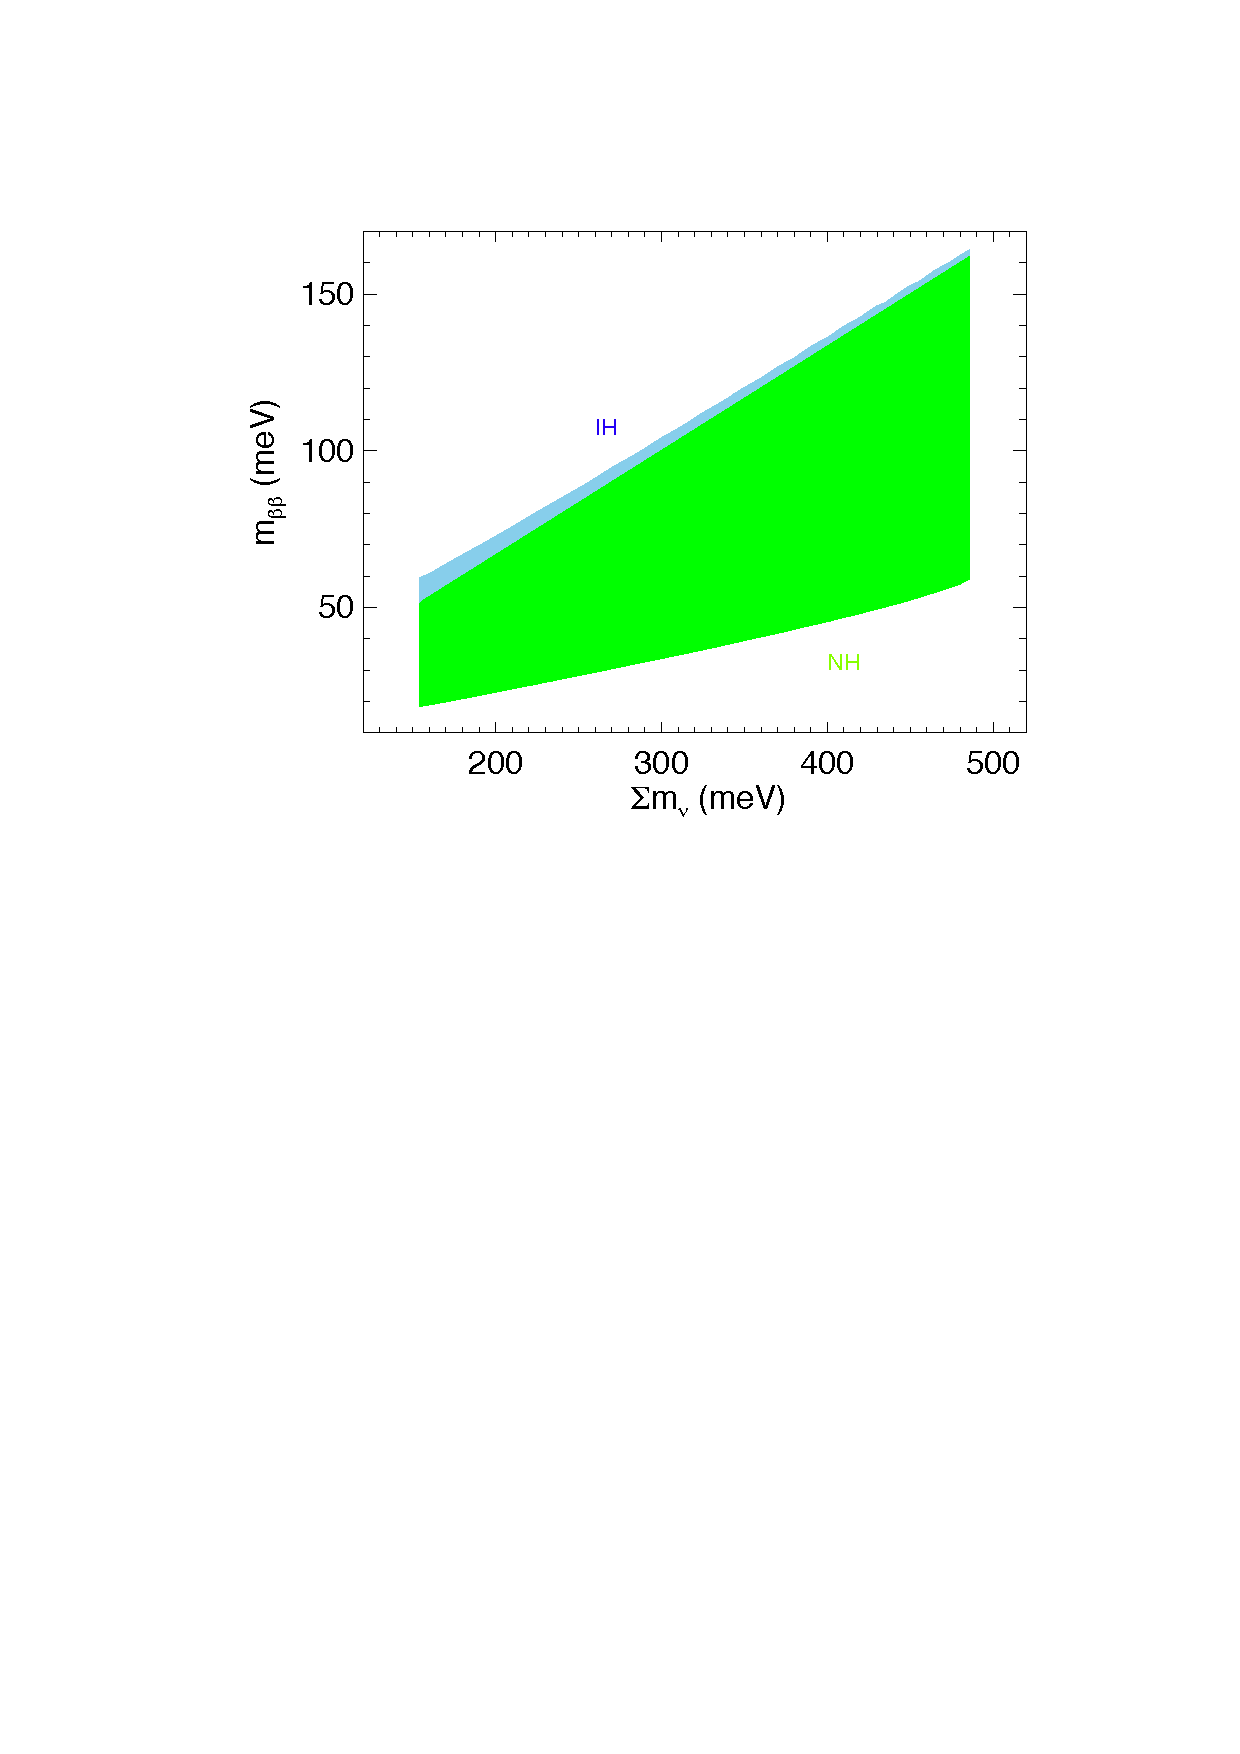
\includegraphics[width=0.65\textwidth]{img/Mbb.pdf}
\caption{The allowed \mbb\ region, as a function of the sum of the neutrino masses, assuming that 
$\sum m_i = 0.32$~eV.} \label{fig.mbb}
\end{figure}
%%%%%%

 Several analyses from recent cosmological results suggest that the sum of the masses of the three neutrinos could be $\sim$ 0.3 eV\footcite{PhysRevLett.112.051303}. The PI and collaborators have demonstrated that, in this case, if the neutrino is a Majorana particle, then, $\mbb \sim [20-150]$~ meV \footcite{GomezCadenas:2013ue}, as shown in Figure \ref{fig.mbb}. In this scenario, the sensitivity of GERDA is outside the ``cosmologically relevant region'' (CRR), while both EXO-200 and KamLAND-Zen would have already explored a significant fraction of CRR {\em for the most optimistic NME set} (while they would be outside CRR for the most pessimistic). 
 
 Clearly, the experimental effort to determine if the neutrino is a Majorana particle, far from being completed is, rather, in its infancy. To establish unambiguously that the neutrino is (or not) a Majorana particle, even in this favourable scenario in which the sum of the neutrino masses is relatively high, experiments must be sensitive to $\mbb \sim 20$~meV, {\em even for the most pessimistic NME} set. On the other hand, a xenon experiment probing a $\Tonu >2.6 \times 10^{25}$~yr, has chances of making a discovery.
 
 
%%%%%%%%%%%%%%%%%%%%%%%%%%%%%%%%%%%%%%%%%%%%%%%%%%%%%%%%%%%%
\subsubsection*{The NEXT experiment and its innovative concepts}
\begin{figure}
\centering
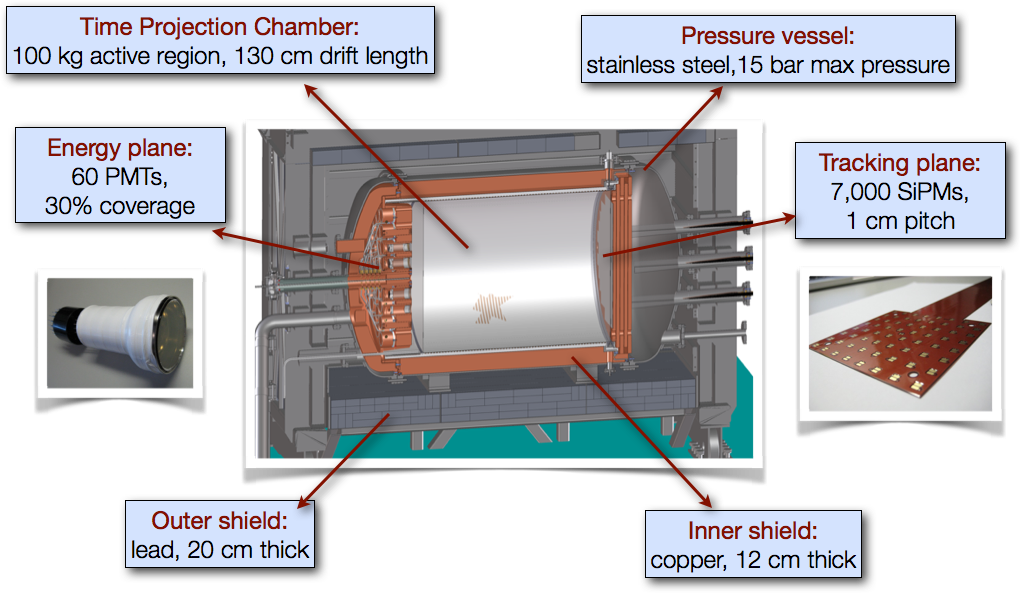
\includegraphics[width=0.9\textwidth]{img/NEXT.png}
\caption{\small A drawing of the NEXT-100 detector showing its main parts.} \label{fig.NEXT100}
\end{figure}

The \emph{Neutrino Experiment with a Xenon TPC} (NEXT)\footnote{\href{http://next.ific.uv.es/}{http://next.ific.uv.es/}} will search for \bbonu\ in \XE\ using  high-pressure xenon gas  time projection chambers (\HPXE). The advantages of the technology are: 
a) {\bf excellent energy resolution}, with an intrinsic limit of about 0.3\% FWHM at \Qbb, close to that of \GE\ detectors; b)
{\bf tracking capabilities} that provide a powerful topological signature to discriminate between signal (two electron tracks with a common vertex) and background (mostly, single electrons); c)
{\bf a fully active and homogeneous detector}, with no dead regions; d) {\bf scalability} of the technique to larger masses; e) the possibility of exciting the barium ion produced in the xenon decay from the fundamental state \TwoS\ to the state \TwoP, using a ``blue'' laser (493.54 nm), and observing the ``red light'' emitted in the transition from \TwoP to \TwoD, thus ``tagging'' the presence of a barium atom in the xenon gas, which cannot be produced by any known background. 

The design of the NEXT chambers is optimised for energy resolution by using proportional electroluminescent (EL) amplification of the ionisation signal. The detection process involves using the prompt scintillation light from the gas as start-of-event time, drifting the ionisation charge to the anode by means of an electric field ($\sim0.3$ kV/cm at 15 bar) where secondary EL scintillation will be produced in the region defined by two highly transparent meshes, between which there is a field of $\sim20$ kV/cm at 15 bar. The detection of EL light provides an energy measurement (in the energy plane, made of PMTs, located behind the cathode) as well as providing tracking through its detection a few mm away from production at the anode plane, via a dense array (1 cm pitch) of 1-mm$^{2}$ SiPMs (the \emph{tracking plane}).

The design of the NEXT-100 detector (Figure \ref{fig.NEXT100}) has been described in a \emph{Technical Design Report}.\footcite{Alvarez:2012haa} NEXT-100 has the structure of a Matryoshka (a russian nesting doll). The outermost layer is a shield made of lead, which attenuates the background from the LSC rock by 6 orders of magnitude (e.g., the \TL\ photons are attenuated from $\sim 10^{12}$~per year to $\sim 10^{6}$~per year). The pressure vessel, built out of steel, can hold 150 kg of xenon at 15 bar. Finally, an inner copper shield, 12 cm thick, constitutes the innermost and more radio-clean layer of the Matryoshka. In addition, all NEXT components have been selected and screened for low background. Of particular importance are the PMTs, whose activity is only 0.4 mBq of \BI\ and 0.3 mBq of \TL\ per unit. Our TDR included a detailed background model. A recent paper has validated these results from measurements in a extensive screening campaign carried out in the past year.\footcite{Alvarez:2012as} Currently, most of the major components entering the NEXT detector have been measured, and those numbers are incorporated in our background model. 

%%%%%%%%%%%%%%%%%%%%%%%%%%%%%%%%%%%%%%%%%%%%%%%%%%%%%%%%%%%%
\subsubsection*{NEXT prototypes}

%%%%%%%%%
%%%%%%%%%
\begin{figure}
\centering
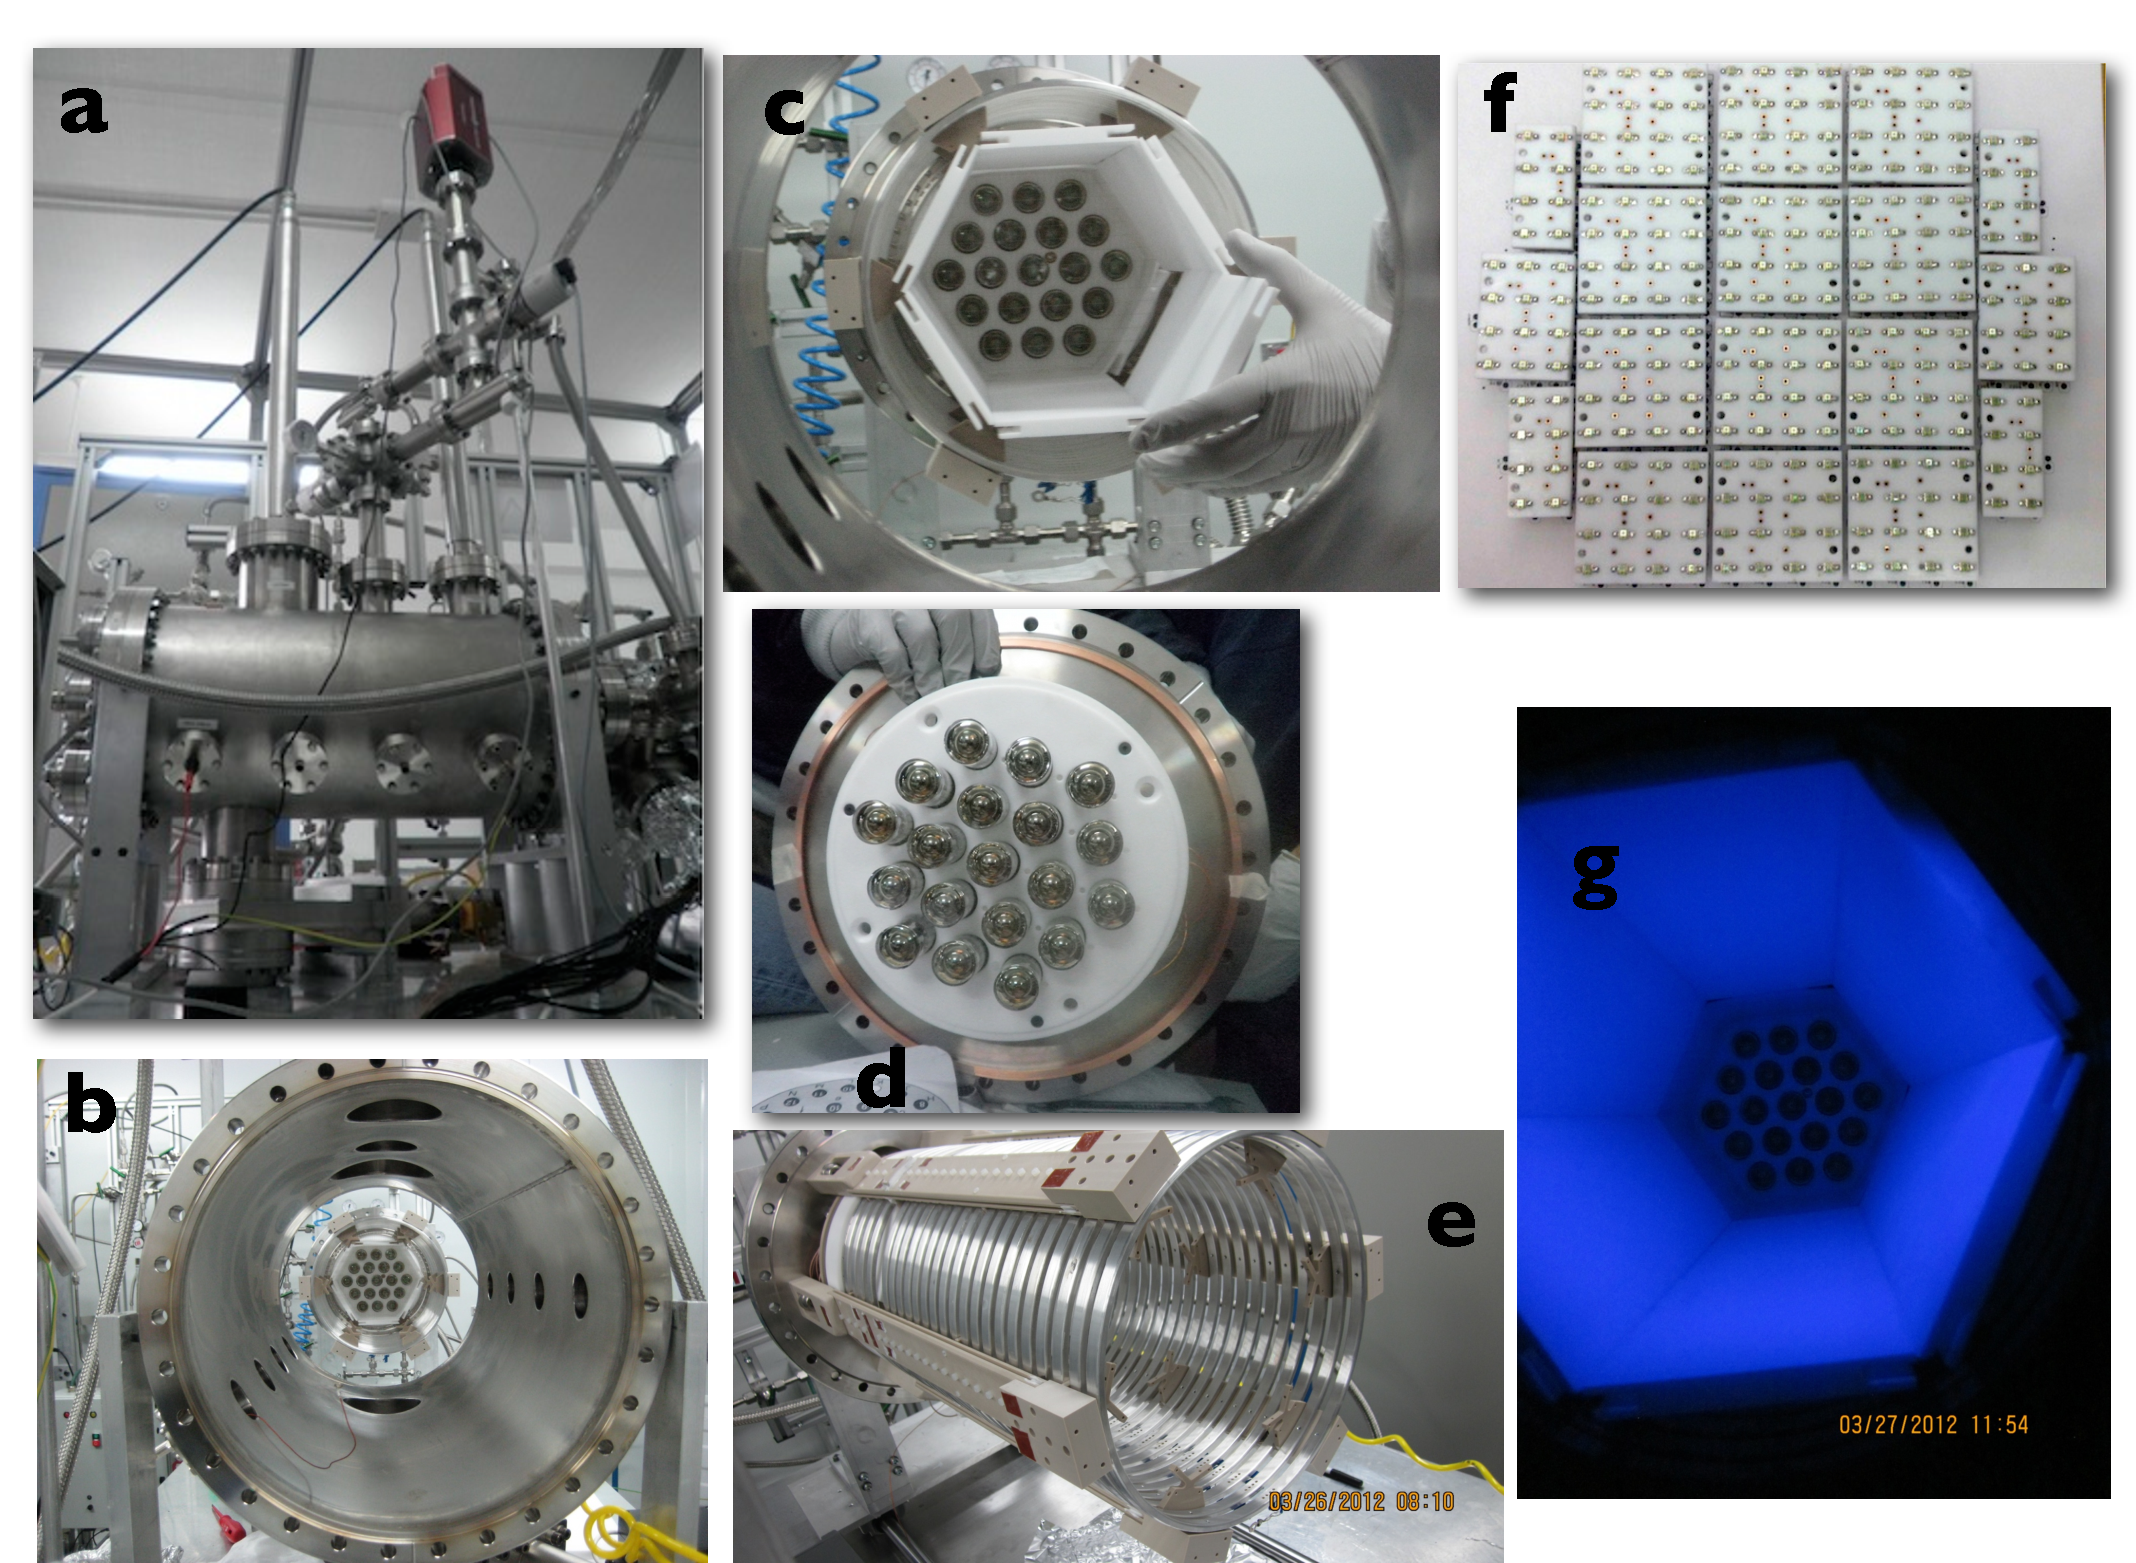
\includegraphics[width=0.7\textwidth]{img/DEMO.pdf}
\caption{\small The NEXT-DEMO prototype. (a) The pressure vessel, showing the HVFT and the mass spectrometer; (b) an expanded view of the detector; (c) Teflon light tube; (d) energy plane, made of pressure resistant Hamamatsu R7378A PMTs; (e) field cage; (f) tracking plane equipped with 300 Hamamatsu MPPCs; (g) Light tube coated with TPB, reflecting UV light in blue.} \label{fig.DEMO}
\end{figure}
%%%%%%%%%%

From 2009 to 2013 the NEXT Collaboration has carried out an intense R\&D program that has culminated in the construction, commissioning and operation of the NEXT-DEMO prototype located at IFIC, and the NEXT-DBDM prototype operating at LBNL. The description of these prototypes and the initial results obtained with them have recently been published\footcite{Alvarez:2012hh, Alvarez:2012nd, Alvarez:2012hu}.

NEXT-DEMO, shown in figure \ref{fig.DEMO}, is as a large-scale prototype of NEXT-100. The pressure vessel has a length of 60 cm and a diameter of 30 cm. The vessel can withstand a pressure of up to 15 bar. The maximum capacity of the detector is 10 kg but in its current configuration (the fiducial volume is a hexagon of 16 cm diameter and 30 cm length) it holds 4 kg at 15 bar. NEXT-DEMO is  equipped with an energy plane made of 19 Hamamatsu R7378A PMTs and a tracking plane made of 256 Hamamatsu MPPCs. 

The detector has been operating successfully for more than one year and has demonstrated: (a) very good operational stability, with no leaks and very few sparks; (b) good energy resolution ; (c) track reconstruction with PMTs and with SiPMs coated with TPB; (d) excellent electron drift lifetime, of the order of 20 ms. In summary, the operation of NEXT-DEMO has been instrumental in the development of the required knowledge to design and build the NEXT detector.

The NEXT-DBDM prototype is a smaller chamber, with only 8 cm drift, but an aspect ratio (ratio diameter to length) similar to the NEXT detector. The device has been used to perform detailed energy resolution studies. NEXT-DBDM achieves a resolution of 1\% FWHM at 660 keV and 15 bar, which extrapolates to 0.5\% at \Qbb.

\subsubsection*{Topological signature}

%%%%%
\begin{figure}
\centering
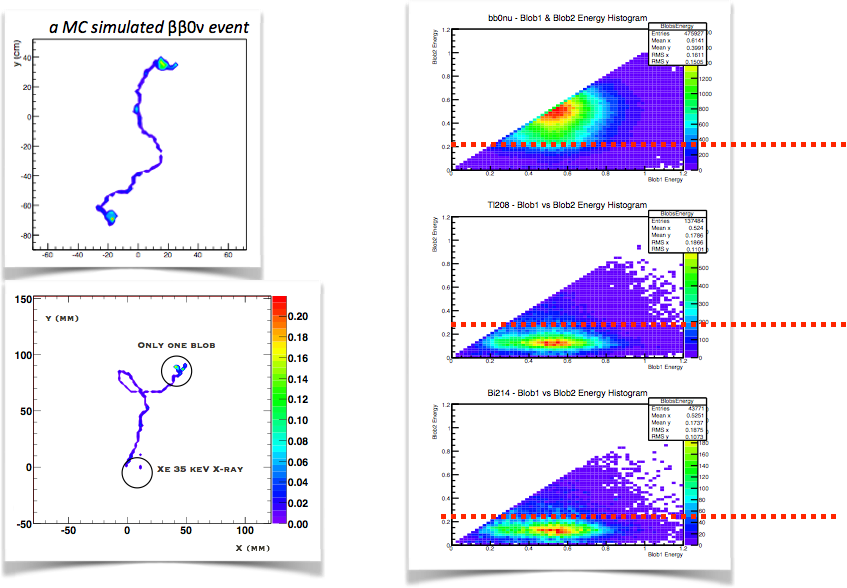
\includegraphics[width=0.9\textwidth]{img/Topology.png}
\caption{\small NEXT has a topological signature, not available in most \bbonu\ detectors. The panel shows the reconstruction of a Monte Carlo signal (topleft) and background (bottomleft) event. The signal has two electrons (two blobs). The background has only one electron (one blob) and the associated emission of a 35 keV X-ray. The color codes energy deposition in the TPC. An scatter plot of the energy of the two blobs shows a clear separation between signal and background regions.}\label{fig.ETRK2}
\end{figure}
%%%%%
	
Double beta decay events leave a distinctive topological signature in HPXe: a continuous track with larger energy depositions (\emph{blobs}) at both ends due to the Bragg-like peaks in the d$E$/d$x$ of the stopping electrons (figure \ref{fig.ETRK2}, topleft). In contrast, background electrons are produced by Compton or photoelectric interactions, and are characterised by a single blob and, often, by a satellite cluster corresponding to the emission of $\sim30$-keV fluorescence x-rays by xenon (figure \ref{fig.ETRK2}, bottomleft).
Reconstruction of this topology using the tracking plane provides a powerful means of background rejection, as can be observed in the figure. In our TDR we chose a conservative cut to separate double--blob from single--blob events which provided a suppression factor of 20 for the background while keeping 80\% of the signal.  

%The NEXT-DEMO prototype has demonstrated that electron tracks can be easily characterised in an HPXe TPC. Na-22 electrons, with an energy of 511 keV, have been used to demonstrate an efficiency of single-blob counting larger than 98\% and a frequency of erroneous double blob counting of less than 0.14\%. This is a robust confirmation of the excellent background rejection capability of the technology. 

\subsubsection*{Energy resolution}

%%%%%%
%\begin{figure}
%\centering
%\includegraphics[width=0.7\textwidth]{imgs2/RES.pdf}
%\caption{Energy resolution measured with NEXT-DBDM prototype at  15 bar. Data points show the measured energy resolution for 662 keV gammas (squares), 30 keV xenon X-rays (triangles) and LED light pulses (circles) as a function of the number of photons detected. The expected resolution including the intrinsic Fano factor, the statistical fluctuations in the number of detected photons and the PMT charge measurement variance. The measured resolution extrapolates to $\sim$0.5\% FWHM at \Qbb.}\label{fig.RES}
%\end{figure}
%%%%%

%%%%%
\begin{figure}
\centering
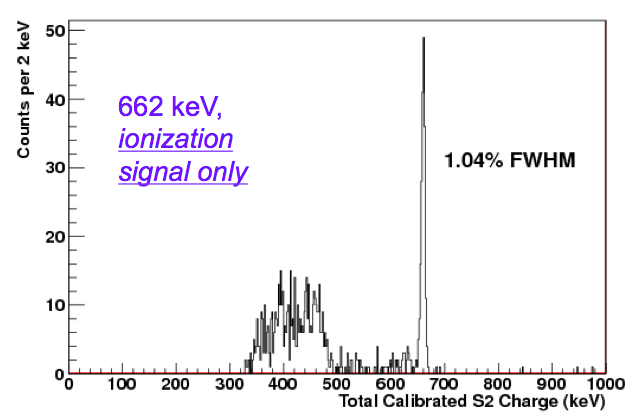
\includegraphics[width=0.6\textwidth]{img/Cs660.png}
\caption{\small The resolution of the photo peak for 662 keV electrons in NEXT-DBDM, at 15 bar is 1\% FWHM (0.5\% FWHM at \Qbb).}\label{fig.ERES}
\end{figure}
%%%%

Figure \ref{fig.ERES} shows the resolution obtained with the NEXT-DBDM apparatus. A resolution of 1\% FWHM with 
662 keV photons, has been measured, which extrapolates to 0.5\% FWHM at \Qbb. This result is not far from the expected limit obtained adding in quadrature the different factors that contribute to the resolution (Fano factor, photoelectron statistics and electronic noise). The resolution measured in NEXT-DEMO extrapolates to 0.7\% FWHM. The difference between both prototypes is due to better photoelectron statistics and aspect ratio in DBDM. The results, are, in any case, better than the target of 1\% FWHM described in the TDR.

The status of the NEXT experiment and the results achieved by the prototypes have been described in a recent
paper \footcite{Gomez-Cadenas:2013lta}.

%%%%%%%%%%%%%%%%%%%%%%%%%%%%%%%%%%%%%%%%%%%%%%%%%%%%%%%%%%%%

\subsubsection*{The NEW detector}
\label{sec.new}

%%%%%%%%%%
\begin{figure}
\centering
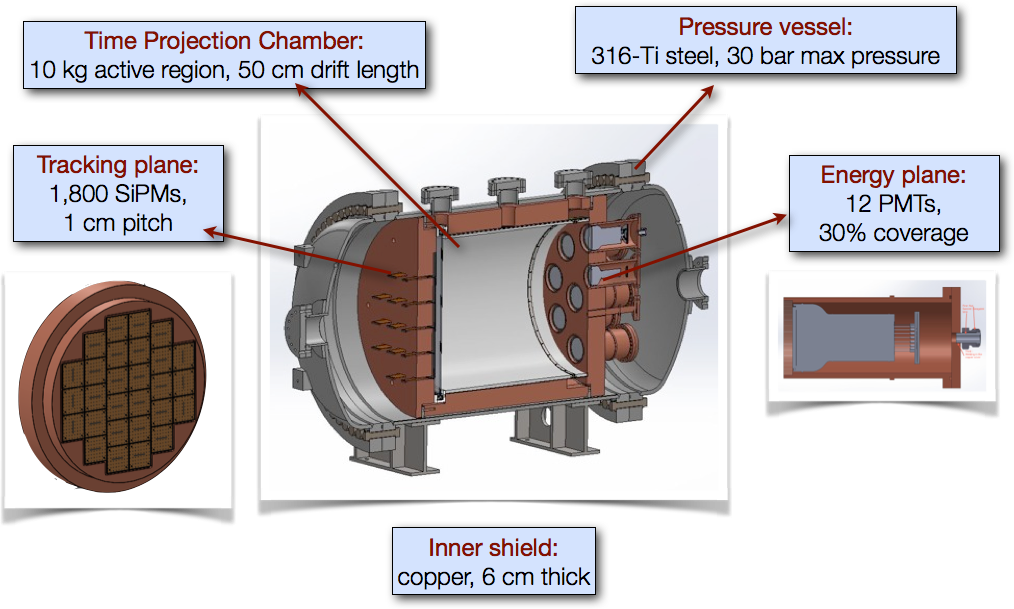
\includegraphics[height=9cm]{img/NEW.png}
\caption{The NEW apparatus.} \label{fig:NEW}
\end{figure} 

The NEW (NEXT-WHITE) apparatus\footnote{The name honours the memory of Professor James White, recently deceased and one of the key scientists of the NEXT Collaboration.}, shown in Figure \ref{fig:NEW} is the first NEXT detector to operate underground. NEW has a triple goal:

\begin{enumerate}
\item {\bf Technology}: it will validate the technological solutions adopted by NEXT-100.
\item {\bf Radiopurity}: it will allow the NEXT collaboration an extra step in the implementation of a radiopure detector.
\item {\bf Physics}: it will demonstrate with measurements of the \BI\ and \TL\ lines, as well as with the measurement of the \bbtnu\ spectrum, the physics capabilities of NEXT-100.
\end{enumerate}

NEW is a scale 1:2 in size (1:8 in mass) of NEXT-100. The energy plane contains 12 radio pure PMTs
of 3 inches diameter, isolated from the gas inside vacuum-tight copper enclosures (we refer to these as PMT cans). The tracking plane technology consists of 30 Kapton Dice Boards (KDB) deploying 1800 SiPMs. The field cage has a diameter of 50 cm and a length of 60 cm. 

The NEXT background model is currently based on a sophisticated Monte Carlo simulation of all expected background sources in each part of the detector. NEW will allow the validation of the background model with the data themselves. Furthermore, it will allow us to identify and correct any possible hot spots, which can only be identified with operating experience.

Furthermore, the calibration of NEW with 
sources of higher energy, will allow a precise study of the evolution of the resolution with the energy. 
In particular it will be plausible to measure the resolution near \Qbb\ using a Thorium source, which provides 2.6 MeV gammas. Last, but not least, we intend to 
reconstruct the spectrum of \bbtnu. Those events are topologically identical to signal events (\bbonu) and can be used to demonstrate with data the power of the topological signature. 

\subsubsection*{Discovery potential of NEXT-100}

The excellent resolution of NEXT (0.5-0.7 \% FWHM) and the combination of low radioactive budget and topological signature (which yields an expected background rate of $5 \times 10^{-4} \ckky$, will allow the NEXT-100 detector to reach a sensitivity on the \bbonu\ period of $\Tonu > 7 \times 10^{25}$~yr for a exposition of 300 kg$\times$yr. This translates in a range for \mbb\ of $[67-187]$~meV. Therefore NEXT-100 will have a substantial chance of making a discovery if the NME is sufficiently high. 

\subsubsection*{Towards a ton-scale high-pressure xenon TPC. BEXT}

%%%%%%
\begin{figure}
\centering
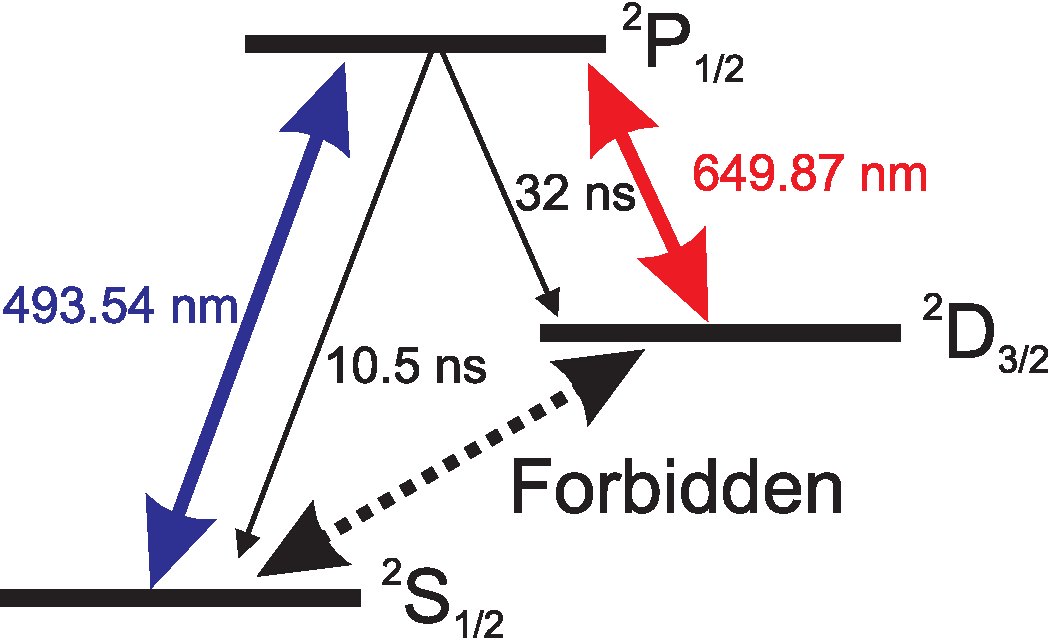
\includegraphics[width=0.65\textwidth]{img/bata.pdf}
\caption{The \BATA\ concept.} \label{fig.BATA}
\end{figure}
%%%%%%

If no discovery is made by the current generation of experiments, the full exploration of the CRR region (corresponding to the inverse hierarchy of neutrino masses) requires detectors of larger mass (at least 1 ton), good resolution and extremely low specific background. The \HPXE\ technology has the potential to provide the most sensitive detector in the ton scale, by scaling the detector to a mass in the range of the ton and adding additional handles to further suppress the background. 

One of the most promising possibilities is to develop the technology to unambiguously tag the barium ion produced in the xenon decay, $Xe \rightarrow Ba^{++} + 2 e$. The conceptual idea to tag $Ba^{+}$ is illustrated in Figure \ref{fig.BATA}. A ``blue'' laser of wavelength 493.54 nm excites (``pumps'') the S state, inducing $S \rightarrow P$~transitions, with a lifetime of $\sim$ 10 ns. About 30 \% of the times the \TwoP\ states decay to the state \TwoD, emitting ``red'' (649.86 nm) fluorescence in a characteristic time of 30 ns. The state \TwoD\ is metastable, but a second laser of suitable wavelength (2051.66 nm) can be used to induce the transition to the ground state (this is known as ``deshelving'').  The whole cycle takes less than 50 ns, and therefore several millions of red fluorescence photons can be emitted by a single ion. 

Of course, the practical application of this beautiful conceptual idea is by no means easy, and in fact, it has been shown to be extremely difficult in liquid xenon by the work of the EXO collaboration. However, it may be feasible in an \HPXE\ detector, where a number of fortunate conditions may occur. These conditions are: a) charge reduction of the emitted barium ion, from $Ba^{++}$~to $Ba^{+}$, which can be induced by collisions with xenon atoms, or by the addition of a suitable quencher, such as TEA, as demonstrated by Sinclair et al\footnote{Sinclair.}, b) ``trapping'' of the barium ion ``in situ'' by the surrounding Xe atoms, which result in a very low drift velocity for the ion; c) location of the ion, done by reconstructing the event vertex. 

All the above needs to be demonstrated with a systematic R\&D program, which must also address many other experimental issues such as pressure broadening of the laser, filtering of Rayleigh scattering, etc. Most importantly, such an experimental program must be carried out by an interdisciplinary group, combining the experience in laser spectroscopy and atomic physics, with the experience in \HPXE\ instrumentation.

The on-going collaboration between the IFIC (and other groups of NEXT) and the Center for Pulsed Lasers (CLPU) \footnote{http://www.clpu.es.}, a national facility dedicated to ultra-intense lasers research and development has made possible to create precisely the interdisciplinary team needed for a successful R\&D program, which can culminate in a ``Barium-tagging Experiment with a Xenon TPC'' (BEXT). We are currently preparing a white paper which describes the theoretical grounds and details the experimental program to be developed\footnote{To be found here}. 

A future detector of 1 ton mass, with a resolution of 0.5 \% FWHM and a background rate in the range of $10^{-6} \ckky$~(thanks to the implementation of barium-tagging) would be able to fully cover the CRR (inverted hierarchy) region in less than 5 years run, assuming a favourable scenario for the NME. Even the most pessimistic scenario could be fully explored, however, with a longer run, since the sensitivity to period increases in this case (virtually background free experiment) linearly with exposure. 

Clearly the construction of a ton-scale \HPXE\ detector implementing a full \BATA\ technology is a very challenging enterprise. On the other hand, we believe that the incremental approach devised by the NEXT collaboration will also work in this case. The construction of the NEW detector is progressing without significant problems thanks to the expertise and know-how gained during DEMO phase, and we expect that NEXT-100 will fully benefit from the experience gained with NEW. Similarly, the \BATA\ technology could be ready in a period of 5-7 years, by approaching the problem step by step. 

To conclude, we have shown that the NEXT-100 detector, which we aim to construct, commission and operate during the next few years has a significant potential of making a major discovery. We have also shown that the \HPXE\ technology with \BATA\ included may be the most promising experimental path to find out if the neutrino is its own antiparticle. 
 

\subsection*{\sc Antecedentes/Previous work}


%Si el proyecto es continuación de otro previamente financiado, individual o coordinado, deben indicarse con claridad los objetivos y los resultados ya alcanzados de manera que sea posible evaluar el avance real que se propone en el nuevo proyecto. Si el proyecto aborda un tema nuevo, deben indicarse los antecedentes y contribuciones previas de los equipos de investigación que justifiquen su capacidad para llevarlo a cabo.
%

This research project is the continuation of the CONSOLIDER-INGENIO project CUP (2010-2014), and the SEIDI project FIS-XXX--- (2012-2014). 

To assess the achievements of the collaboration so far it is useful to review the historical development of the project. 

The largest HPXe chamber ever operated in the world before NEXT was the so-called St.~Gotthard TPC \footcite{Luscher:1998sd}. It had a total mass of 5 kg of xenon, and was, therefore, of a similar size as our NEXT-DEMO prototype, although it operated at a considerably lower pressure (5 bar). Furthermore, the St.~Gotthard TPC amplified the ionisation charge ---needed to measure the event energy--- with a plane of wires at high voltage. This classical technology, the only one mature enough in the mid 90's, when the experiment operated, required the addition of a quencher ($CH_4$) to the xenon, to avoid sparks. Unfortunately, the methane destroyed the scintillation signal in xenon, with two undesirable consequences: a) the possibility to measure the start-of-the-event or $t_0$, defined by the prompt scintillation signal was lost; and b) the measurement of the energy resolution degraded. The energy resolution of the St.~Gotthard TPC was 7\% at \Qbb\ and the background was dominated by events coming from the detector walls that could not be vetoed due to the lack of $t_0$. The (relatively) poor results obtained with this early experiment, prompted the EXO experiment to choose liquid xenon and abandon the \HPXE\ technology. However, a LXe TPC has mediocre resolution, due to abnormal partition between scintillation and ionisation in the liquid phase (EXO-200 measures 3.6\% FWHM at \Qbb) and the topological signature of the event (the track of the two electrons) is also lost due to the high density of the liquid. 

The first problem that the NEXT project faced was to develop the technology to build high-pressure, radio-pure xenon chambers. High-pressure implies also moderately high-vacuum, needed for gas purity. The technology did not exist in Spain, and was rather underdeveloped elsewhere. All the \HPXE\ detectors built prior to 2009 (except for the St.~Gotthard TPC) where small objects, typically holding a few hundred grams of gas at moderately low pressures. Radiopure copper, as in the St.~Gotthard TPC, could not be used to build the pressure vessel, since the NEXT-100 detector was much larger and had to hold much higher pressures.  It was necessary, therefore, to find a radiopure solution for the pressure vessel, either in steel or in titanium (an alloy of steel and titanium was chosen at the end). Furthermore, it was necessary to develop a way to read the ionisation signal without killing the scintillating signal (i.e. without using quenchers) and without degrading the excellent intrinsic resolution available in the gas. 

The construction of the NEXT-100 detector faced, therefore, a large number of challenges. From the instrumental point of view, it was necessary:

\begin{enumerate}
\item {\em To acquire the technology}. This required equipping state-of-the-art laboratories, hiring specialised personnel and building prototypes.
\item {\em To study technological solutions, in order to read the ionisation and scintillation signals}. A number of possibilities were, a priori, available. In particular, the ionisation charge could be transformed in secondary VUV light and be read with optical sensors (the EL solution), or amplified with micro-pattern devices (the micromegas or MM solution). Within the EL solution, there was the choice of using photomultipliers (PMTs) and multi-pixel (SiPMs) devices or avalanche photo diodes (APDs). 
\end{enumerate}

Coupled with those instrumental challenges, the collaboration had to attack major mechanical engineering problems:

\begin{enumerate}
\item{\em Design and build a radiopure pressure vessel}, capable of holding at least 100 kg of xenon and capable of withstanding up to 15 bar with negligible losses (less than 1 gram a year). 
\item{\em Design and build a radiopure energy plane}, capable of protecting the PMTs inside the pressure vessel.
\item{\em Design and build a radiopure tracking plane}, including large custom feedthroughs, needed to extract the signals of $\sim$ 8000 SiPMs from the pressure vessel. 
\item{\em Design and build a state-of-the-art gas system}, capable of guaranteeing gas purity via continuous recirculation in a hermetic loop. The gas system had to guarantee redundancy and safety to minimise to negligible level the chances of loosing any substantial amount of enriched xenon gas. 
\item{\em Design and build the shielding of the detector}, choosing between several possible solutions (e.g., a water tank or a lead castle).
\item{\em Design and build the infrastructures} to hold the apparatus (working platform, seismic pedestal).
\end{enumerate}

Finally, one had to provide solutions for the electronics of the PMTs and the SiPMs, the  DAQ and the software.

In the years 2010-2013, the various problems were attacked in a systematic way: a brief summary can be jotted down as follows:

\begin{enumerate}
\item {\em Learning R\&D period (2010)}, needed to acquire the very innovative technology the detector is based on, and to equip state-of-the-art laboratories in some of our participating institutions. This phase of the project resulted in the construction of several prototypes, including NEXT-DEMO, capable of holding up to 4 kg of gas (thus, the same mass than  the St.~Gotthard TPC, and much higher pressure). DEMO has been operating continuously at IFIC for more than two years, demonstrating, in addition to its excellent performance the stability of the technology.  

\item {\em Selection R\&D period (2011)}, targeted to choose among the various technological solutions candidate to be implemented in NEXT-100. This period culminated in June of 2011 with the presentation of a Conceptual Design Report (CDR), where the NEXT detector was defined as an electroluminescent HPXe TPC equipped with photomulitpliers (PMTs),  to read the event energy and multipixel proportional counters (MPPCs also called SiPMs), to reconstruct the event topology. 

\item {\em R\&D targeted to produce a Technical Design Report (TDR)}, which defined the actual detector to be built. The TDR was presented in February 2012 and in final version in May 2012. The TDR defined solutions for the instrumentation, mechanical design of detector and infrastructures, electronics, DAQ and software, as well as the detector background model. 

\item {\em Demonstration of performance}: during 2012 and 2013, the results of the prototypes were analysed and published, showing the excellent performance (energy resolution, electron reconstruction) of the apparatus, as well as the robustness of the EL technology \footnote{http://next.ific.uv.es/next/talks.html}.  
\end{enumerate}

To summarise, the previous work of the NEXT collaboration has resulted in the demonstration, using large prototypes (NEXT-DEMO/DBDM ) of the excellent performance of the \HPXE\ technology. Furthermore, the full detector design has been detailed in the TDR and an exhaustive radiopurity campaign has been carried out  validating the background model assumed in the TDR.  The physics case of NEXT has therefore been clearly established, demonstrating that this technology has the potential to be one of the very few that can be extrapolated to the ton scale.\footcite{GomezCadenas:2012jv} 



\subsection*{\sc Objetivos/Objectives}

\subsection*{Objectives}

%2. La hipótesis de partida y los objetivos generales perseguidos con el proyecto coordinado en su conjunto, así como la adecuación del proyecto a la Estrategia Española de Ciencia y Tecnología y de Innovación y, en su caso, a Horizonte 2020 o a cualquier otra estrategia nacional  o internacional de 

The overall goal of this research proposal is the construction, commissioning and operation of the NEW and NEXT-100 detectors, during a period of 4 years, from 2015 to 2019, through the following objectives.  

%%%%%
\begin{figure}
\centering
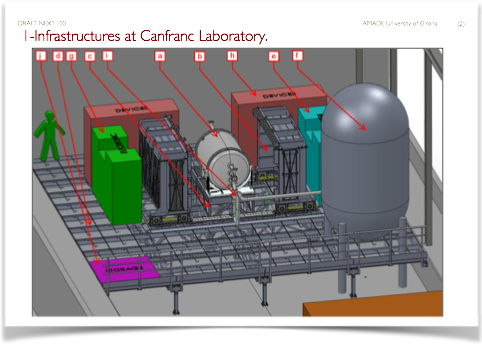
\includegraphics[width=0.9\textwidth]{img/InfraStructures.png}
\caption{\small The infrastructures at Canfranc include: working platform, seismic pedestal, lead castle, gas system, emergency recovery system, radon suppression system and clean tent.}\label{fig.INFRA}
\end{figure}
%%%%

%%%%%
%\begin{figure}
%\centering
%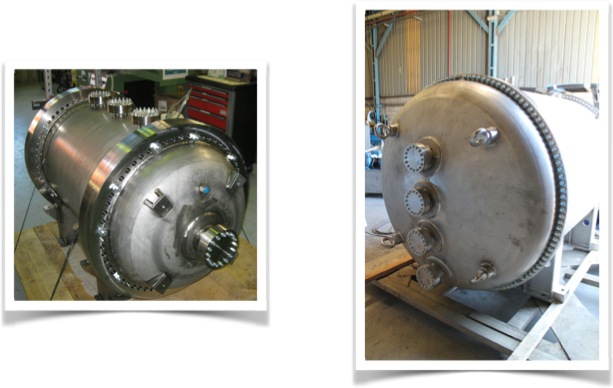
\includegraphics[width=0.9\textwidth]{img/PV.png}
%\caption{\small The NEXT pressure vessels, made of radio pure titanium-steel alloy and capable to withstand up to 25 bar pressure. Left, the NEW PV. Right, the NEXT-100 PV.}\label{fig.PV}
%\end{figure}
%%%%

%%%
\begin{enumerate}
\item {\bf Complete the needed infrastructures to operate NEW and NEXT-100 at the LSC} (Figure \ref{fig.INFRA}). The activity related with this objective has started already in 2014. The working platform, seismic pedestal and lead castle are already installed at the LSC, and the equipment related with the gas system and emergency recovery system has been purchased using AdG/ERC funds and will be installed at the LSC in the first quarter (Q1) of 2015. The radon suppression system is a major equipment, which has been requested by the LSC as a part of its infrastructures. The clean tent is necessary to operate in a clean environment and needs to be in place also in the first quarter of 2015. For this reason, it will be purchased also with AdG funds. 

\item {\bf Complete the construction of NEW}. The current plan foresees to assemble the detector for a preliminary test at IFIC in the fourth quarter (Q4) of 2014. After validating basic operation the detector will be disassembled. Part of the pieces (pressure vessel, copper shield, and the copper support plates of the energy plane and tracking plane) will be sent to the LSC, where they will undergo a specialised cleaning procedure designed to eliminate any traces of surface radioactivity. The field cage and the PMT enclosures (PMT ``cans'') will be sent to the Gran Sasso Underground Laboratory (LNGS), for cleaning and coating with wavelength shifters (TPB). The detector will be fully assembled at the LSC in the second quarter (Q2) of 2015. The full construction of NEW is financed by the the AdG grant. 
 
\item {\bf Commissioning of NEW}, which implies extensive testing to certify safe and stable operation (no leaks, no sparks), as well as testing and integration of all the subsystems. This period requires extensive presence of scientific and technical personnel at the LSC. We expect to complete commissioning in the third quarter (Q3) of 2015.

\item {\bf Evaluation of Performance}. During the fourth quarter (Q4) of 2015, we will evaluate the performance of the detector, once the commissioning is concluded. Such evaluation will allow us to correct for design problems (if they arise) or to introduce improvements in the engineering (if needed). We will also assess the overall radioactive budget of the detector, to ensure the absence of ``hot spots'' (excess of radioactivity introduced accidentally in the detector). 

\item {\bf NEW physics run}. During 2016, we will operate continuously the NEW detector at the LSC. The physics runs of NEW has several goals: a) measurement, using radioactive sources, of the energy resolution as a function of the energy, and in particular at \Qbb; b) measurement, using radioactive sources, of single (``background'') electrons, as well as ``double electrons'' (produced by the double escape peak of Tl-208, and used to characterise the signal); c) measurement of the standard mode \bbtnu; and d) a full measurement of the spectrum, after selection cuts, thus quantifying, from the data themselves, the background model. Notice that all the above measurements can be directly extrapolated to NEXT-100, since the scale between both detectors is just 1:2. 
%

\item {\bf Construction of NEXT-100}. The construction of NEXT-100 will proceed through 2015 and 2016. In fact, the pressure vessel has already been built, and other mechanical parts (inner copper shielding, and support plates) will also be built in 2015. The field cage, energy plane and tracking plane will be built in 2016, after the evaluation of performance of NEW. The energy and tracking plane will be built in Spain, while the field cage will be built in the USA.

\item {\bf Commissioning of NEXT-100}. The commissioning of NEXT-100 will benefit from the experience gained commissioning and operating NEW. We consider feasible to commission the detector during the first 2 quarters of 2017, but our project management plan allows for two extra quarters. The main reason is to guarantee enough time to run with normal xenon before circulating the precious (and very expensive) enriched xenon in the gas system and the detector. Notice that the detector can be fully calibrated, and the backgrounds can be characterised with normal xenon (in fact, this is a good strategy, since one has the guarantee that there is no signal in the data).  

\item {\bf Physics run of NEXT-100}. The physics run may start in the third quarter of 2017, but the project plan foresees the first quarter of 2018. After one year of run, NEXT-100 should reach the sensitivity of the current leading experiments. We currently foresee to run for three years (2018 to 2020), achieving a sensitivity to \mbb\ that makes a discovery possible if NME are sufficiently large and the neutrino is a Majorana particle. 

\item { \BATA\ \bf R\&D}: The development of the project indicates that NEXT could be upgraded to the ton scale, and its performance boosted using barium tagging in 2020. This implies two different R\&D periods. From 2014 to 2018, we aim to demonstrate the feasibility of the technology, performing a systematic set of (small) experiments. During the period 2018-2020, while NEXT-100 takes data, we aim to reuse the NEW detector to construct a large scale prototype of a \HPXE\ with \BATA. 

\end{enumerate}

This project will allow us to complete the second and third phases of the NEXT experiment, with the construction and operation of NEW and NEXT-100.  It is important to remark that NEXT is the only large experiment in particle physics fully carried out in Spain. NEXT makes full use of the LSC facilities, boosting also its international relevance.  NEXT is a CERN recognised experiment and has been listed by NSA\footnote{http://science.energy.gov/~/media/np/nsac/pdf/docs/2014/NLDBD\_Report\_2014\_Final.pdf} as one of the key \bbonu\ experiments in the field, and the one with best future prospects. It has been supported by a CONSOLIDER-INGENIO. It brings a major contribution to the spanish program for science, including the possibility of making or participating in a fundamental discovery. The support of the AdG/ERC makes it clear that the projects suits perfectly well the goals of H2020.


\subsection*{\sc Adecuación al programa de Retos de la sociedad/ Idoneity to the program of challenges of society  }

%Si la memoria se presenta a la convocatoria de RETOS INVESTIGACIÓN, deberá identificarse el reto cuyo estudio se pretende abordar y la relevancia social o económica prevista.
%
This research project is presented within the program of ``Challenges of society'', specifically, challenge number 6: {\bf Change and social innovation.}

We argue that this project represents a major innovation in the way that particle physics is conducted in Spain, and thus marks a path to a more productive approach to research.

Particle physics is a clear example of the so-called ``big-science'',
characterised by the need for large budgets, big machines (such as particle accelerators) and large staffs (for example, the number of physicists participating in the ATLAS and CMS experiments is of the order of 5,000). The discovery of the Higgs boson is a quintessential of such big science, and clearly exemplifies its pros and cons. The obvious pro is the major scientific achievement that the discovery represents. Such a discovery has required the construction and operation of the LHC, one the most impressive scientific machines ever built by humankind. The gargantuan scale of the effort could only be met by a collective effort centralised in the largest particle physics laboratory in the World, CERN.  

Among the cons of big science are the large budgets that it involves, often invested in purchasing equipment to be installed at CERN (or other laboratories) and in paying scientific staff whose activity also develops at CERN. Such large budgets are often justified in terms of industrial and scientific returns. While those returns certainly exist, it is often not easy to quantify their impact in the countries that finance big science. Scientific authorship is one example. It is difficult to assign credit, in particular to students and young post-docs, when the detector is built and operated by thousands of physicists, all of them signing, normally in alphabetic order, the scientific papers. Furthermore, returns tend to be larger for countries who are already very developed scientifically. Specifically, the positions of leadership in the large CERN experiments, and in the CERN scientific and technical divisions, are dominated by countries like Germany, Switzerland, U.K., France and Italy. Industrial returns also tend to be larger for those countries. Instead, the scientific and industrial returns for Spain are very modest. 

Remarkably, the countries leading the big science at CERN and other laboratories have also developed ``national science'' physics programs. A case of great interest is Italy, a country not very different from Spain, in terms of GDP and social habits. However, the international impact and the returns of physics in Italy is much larger than in Spain. For example, the number of Spanish staff members at CERN is 115, to be compared with 275 corresponding to Italy (which has the second largest staff population, after France, with 1031 and followed by UK, with 223). Adding fellows and associates (that is, temporary CERN contracts), the figures for Spain are 363, to be compared with 1726 for Italy\footnote{\href{http://council.web.cern.ch/council/en/Governance/TREF-PersonnelStatistics2012.pdf}{http://council.web.cern.ch/council/en/Governance/TREF-PersonnelStatistics2012.pdf}}. Several italians have served as CERN general directors, and have led or are leading the major experiments, such as ATLAS and CMS. The next CERN general director (and perhaps the first woman to occupy such position in the history of the lab) may be the ex-spokesperson of ATLAS, the italian physicist Fabiola Gianotti. Moreover, Italy has four Nobel prizes in physics (Marconi, 1909, Fermi, 1938, Segrè 1959, Rubbia 1984), while Spain has none. 

Remarkably Italy also boasts the best underground laboratory of Europe, and one of the best of the world, the LNGS. The lab hosts 20 experiments including three experiments searching for \bbonu\ processes (GERDA, CUORE and COBRA) and two experiments searching for Dark Matter (WARP and EXO). 

Through these experiments, the italian physics attracts external talent (some of the best physicists from Europe and USA participate in experiments at LNGS) and external funding, complements the big science at CERN with physics of a smaller scale concerning human resources and budgets (the \bbonu\ experiments typically include about 50-100 physicists, including Ph.D. students, to be compared with $\sim 3,000$~of ATLAS or CMS, and the budgets are one order of magnitude smaller). However, such ``local'' physics results in discoveries of great scientific impact (such as the discovery of neutrino oscillations, which has been the result of a world-wide effort involving underground laboratories in Italy, USA, Canada, Russia and Japan). It also allows the training of students and post-docs in experiments where young physicists can made a major impact at all levels, ranging from the construction of the detector to the analysis of the data (this is to be contrasted with the large and hyper-specialised efforts at CERN, where students and post-doc are often restricted to very specific areas of the experiment). Last, but not least, such local science has an important impact in the italian industry and in the appreciation of science by the public in general. 

We argue that, in order to balance and optimise the current big-science effort in Spain, it is necessary to develop the physics of the LSC, in analogy to the italian case. NEXT is the flagship experiment of our national laboratory, and has achieved intentional recognition, as demonstrated by the fact that is a recognised CERN experiment and has obtained an AdG/ERC, the first grant of this type in the field of particle physics. 

We, therefore, consider that the NEXT project is a clear example of social innovation, as it has the potential of implementing profound changes in spanish physics. As described in this project, NEXT, through its various stages, can hit a major discovery. It will bring international credit and visibility to our science and to the LSC. And it has an important impact both in local industry (through contracts to many national firms, and development of high technology) and in the public perception of science (thorough a very intense activity in public forums including large-circulation cultural magazines such as JotDown, where the PI of this project directs the science section). 

Furthermore, the on-going collaboration with the CLPU further reinforces the above arguments, since the effort involves now a second national scientific installation. In addition, the \BATA\ program implies a major example of inter disciplinarity, and can result in a number of important technological returns (development of micron laser technology, which can be applied to molecular fluorescence, among other examples).

It is important to remark that, while the usual operation of big-science in Spain implies to finance the participation of our groups in labs like CERN (including the annual CERN quota, the common-fund of the experiments and the contributions to construction and operation of the CERN experiments), the national science that NEXT represents obtains external funding through ERC projects (including the AdG and several H2020 actions currently in progress involving LSC), as well as the contributions of the international collaboration (in particular, in the case of NEXT through the USA groups led by Prof. Dave Nygren, the inventor of the technology in which NEXT is based and a major driving force of the experiment) to detector construction and operation. NEXT also attracts external talent to our country (as the intense collaboration with top USA universities demonstrates). The NEXT group is very international, and several of our post-docs are of have been financed by EC grants (such as the Marie Curie). 

Last but not least, the NEXT experiment, and in particular the collaboration with the CLPU, involves the extensive development of photonics listed as one of the  "Facilitating Essential Technologies".


\subsection*{\sc Objetivos subproyectos/ Objectives of subprojects}

\subsubsection*{Objectives of the COORD subproject}
The COORD subproject leads objective 1 (completion of infrastructures),
objective 3 (commissioning of NEW), and objective 7 (commissioning of NEXT-100). It co-leads, together with the ENG subproject objective 2 (NEW construction) and objective 6 (construction of NEXT-100). It co-leads objectives 4 and 7 (evaluation of performance of NEW and NEXT-100) together with CALREC and co-leads objective 9 (\BATA\ R\&D) together with CLPU.

The ENG subproject leads the development of the electronics of the NEW and NEXT-100 detector (objectives 3 and 6). Evaluation of the detector performance requires both an extensive calibration and a well tuned reconstruction, areas lead by the CALREC subproject. All the sub projects will participate in the \BATA\ R\&D. CLPU will bring in the laser technology, COORD the construction of the prototype chambers, ENG the deployment of sensors and electronics and CALREC the reconstruction of events. The participation of CLPU (BATA subproject) is essential for this objective.

Next we describe with more detail the objectives of each subproject.


The objectives of this coordinated project correspond to the Working Packages described in the NEXT Project Management Plan (PMP). Specifically: 
\begin{itemize}
\item {\bf WP1: PV (Pressure Vessel)}: Construction of the NEW and NEXT-100 pressure vessels. 
\item {\bf WP2: GS (Gas System)}: Installation and commissioning of the Gas System for NEW and NEXT-100 at the LSC. 
\item {\bf WP3:IS (Infrastructures)}: Construction of the infrastructures (working platform, seismic pedestal, lead castle, radon suppression system and clean tent), needed for the operation of NEW/NEXT-100.
\item {\bf WP4: FC (Field Cage)}: Construction of the field cage, light tube, HVFT and EL grids of NEW and NEXT-100.
\item {\bf WP5: EP (Energy plane)}: Construction of the NEW/NEXT-100 energy planes.
\item {\bf WP6: TP (Tracking plane)}: Construction of the NEW/NEXT-100 tracking planes.
\item {\bf WP7: FEE (Front-End electronics)}: Front-End electronics of energy and tracking planes.
\item {\bf WP8: DAQ (Data Acquisition )}: Data  acquisition of the energy and tracking planes.
\item {\bf WP9 ONL (Online) }: Online monitoring for NEW/NEXT-100. 
\item {\bf WP10: SLW (Slow Controls)}: Slow controls of the detectors, gas system and ancillary systems.
\item {\bf WP11: MC (Monte Carlo)}: Monte Carlo simulation of the detector(s) and implementation of the background model. 
\item {\bf WP12: REC (Reconstruction)}: Offline reconstruction of events in NEW/NEXT-100.
\item {\bf WP13: SOF (Software)}: Development and maintenance of software tools (reconstruction and analysis frameworks, release tools, software libraries) and coordination of data and Monte Carlo productions. 
\item {\bf WP14: CAL (Calibration)}: Calibration of the NEW/NEXT-100 with radioactive sources. 
\item {\bf WP15: RAD (Radiopurity)}: Screening, using the LSC facilities, as well as several other techniques, of all the components being used in the  NEW/NEXT-100 detectors. 
\end{itemize}

The COORD subproject addresses the objectives corresponding to WP1 to WP6, WP11 and WP13. The objectives of the ENG subproject are those corresponding to WP7 to WP10. The objectives of the CALREC subproject are those included in WP12 and WP14. Finally, the objectives of the RPUR subproject are those included in WP15.  


% Los objetivos específicos de cada uno de los subproyectos participantes, enumerándolos brevemente, con claridad, precisión y de manera realista (acorde con la duración prevista del proyecto).
%
% En los subproyectos con dos investigadores principales, deberá indicarse expresamente de qué objetivos específicos se hará responsable cada uno de ellos.
%

\subsubsection*{Objectives of the COORD subproject}

\begin{figure}
\centering
\includegraphics[height=8cm]{img/LeadCastle.jpg}
\caption{The working platform, seismic pedestal and lead castle, in open configuration, at the LSC.} \label{fig:INFRA}
\end{figure}


\begin{figure}
\centering
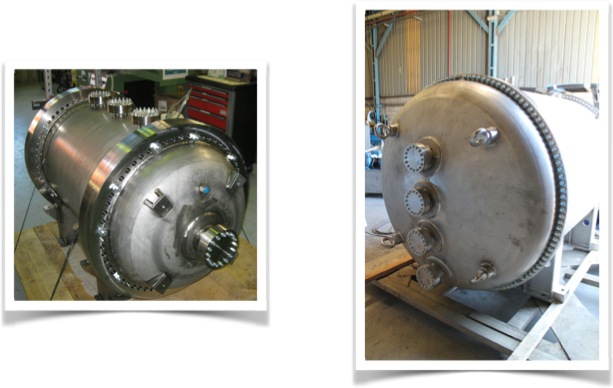
\includegraphics[height=8cm]{img/PV.png}
\caption{The pressure vessel of NEW (left) and NEXT-100 (right).} \label{fig:PV}
\end{figure}

%%%%%
\begin{figure}[t!b!]
\begin{center}
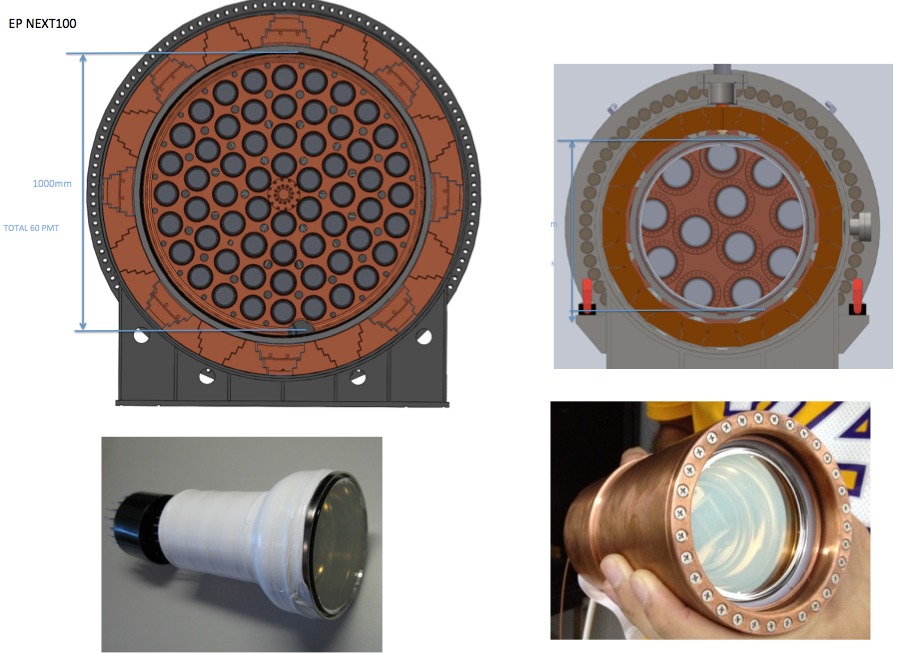
\includegraphics[width=.9\textwidth]{img/EPNext-100.png}
\end{center}
\caption{Top left: NEXT-100 energy plane (60 PMTs). Top right: NEW energy plane (12 PMTs).
Bottom left: The R11410-10 PMT from Hamamatsu; bottom right: a PMT can prototype.} \label{fig:EnergyPlane}
\end{figure}

%%%%%%%
%\begin{figure}[tbhp!]
%\begin{center}
%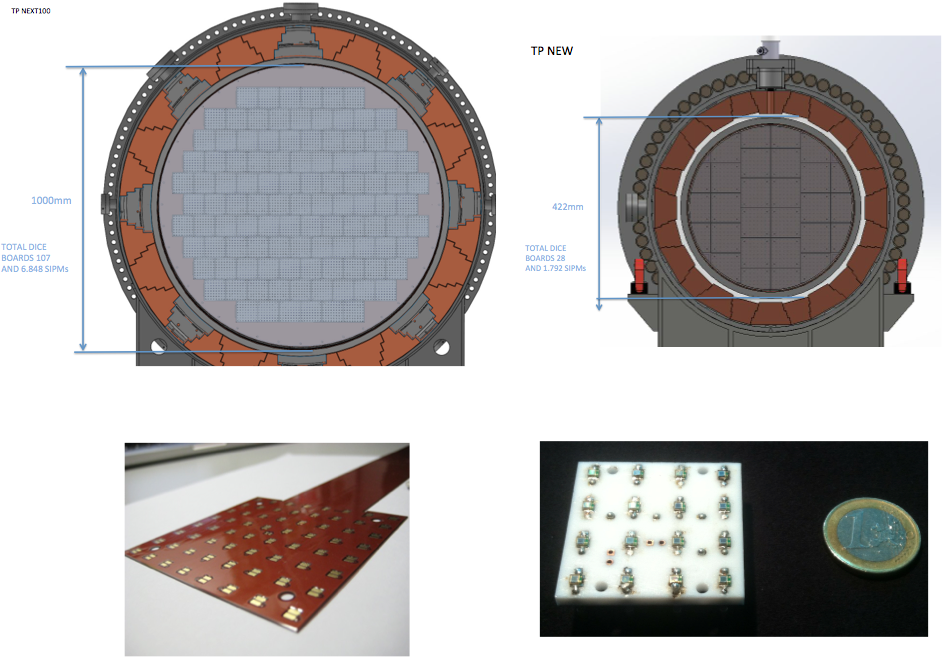
\includegraphics[width=0.7\textwidth]{img/TPNext-100.png}
%\end{center}
%\caption{Top left: the tracking plane of NEXT-100, will deploy 107 of the newly developed Kapton Dice Boards (KDB) shown in bottom left (64 SiPM per KDB, no connector, low noise tracing, low radioactivity). Top right: NEW will deploy about 20\% of the KDBs (28). Bottom right: the Cuflon Dice Board containing 16 (4$\times$4) SiPMs used for DEMO. The KDB improves dramatically the technology.} 
%\label{fig.db2}
%\end{figure}
%%%%%%%

The specific objectives of the COORD subproject are:

\begin{enumerate}
\item {\bf Complete the needed infrastructures to operate NEW and NEXT-100 at the LSC}. 
The infrastructures include: a) working platform and seismic pedestal; b) lead castle; c) gas system; d) clean tent; e) radon suppression system. 
\begin{enumerate}
\item The working platform, seismic pedestal and lead castle are already installed at the LSC (Figure \ref{fig:INFRA}).
\item The equipment related with the gas system and emergency recovery system has been purchased during 2014. The gas loop and compressors will be installed at the LSC during the first quarter of 2015 (Q1'15). The emergency recovery system will be installed during the second quarter 2015 (Q2'15). The clean tent and radon suppression system will also be installed during Q2'15. 
\end{enumerate}

\item {\bf Construction of NEW}, foreseen to be completed in Q2'15, and involving:
\begin{enumerate}
\item {\em Construction of the NEW pressure vessel (NPV)}.
The NEW and NEXT-100 pressure vessels, shown in Figure \ref{fig:PV} were designed to withstand pressures in excess of 20 bar, and to operate with negligible losses at 15 bar. They are built using a 316Ti alloy of low activity ($\sim$0.2 mBq/kg for the thorium series and the uranium series, as measured by our screening campaign). 

The design of the PV was a collaboration between IFIC and LBNL groups. They have been manufactured by several Spanish companies (TRINOS, MOVESA and ACYM) and has benefited from a CEDETI grant. Currently (Q4'14) the NEW pressure vessel (NPV) is being fitted with a copper shield (called the Inner Copper Shield, ICS) that attenuates residual ambient radiation. NPV will be shipped tested for functionality at IFIC in Q1'15, then shipped to LSC and commissioned during Q2'15. 

\item {\em Construction of the NEW field cage (NFC)}
The NEW field cage (NFC) produces an uniform electric ($\sim$ 300 V/cm) field inside the  detector that drifts the ionisation electron to the anode, where they are further accelerated in the electric field produced between a pair of transparent grids, called the electroluminescent (EL) grids. 

The main body of the field cage is a high density polyethylene (HDPE) cylindrical shell with a 2.5\,cm wall thickness.  The drift region will consist of radiopure  copper strips connected with low radioactivity resistors.  The light tube consists of thin sheets of teflon, coated with tetraphenyl butadiene (TPB) wavelength shifter to shift the UV light produced in xenon to the blue region (PMT and SiPMs operate best in this region, around 450 nm).  A high-voltage feedthrough (HVFT) in the cathode and another one in the anode, allow the definition of the voltages. The cathode HVFT is designed to withstand up to 100 kV, and the HVFT of the anode to withstand up to 40 kV. The design of the HVFT, identical for NEW and NEXT-100 improve those that were built for DEMO by the Texas A\&M group. The field cage and grids of NEW and NEXT-100 are also identical, to a scale 1:2. The grids use a stainless steel mesh with pitch 0.5 mm and wire diameter 30 microns, which results in an open area of 90\%.  

The construction of NFC is currently under way (Q4' 2014). The HDPE body is being manufactured by the AIMPLAS company. The HVFT and the grids are being manufactured at Texas. The  NFC will be tested at IFIC before shipping to the LSC in Q1'15. Installation and commissioning at the LSC will occur in Q2'15. 

\item {\em Construction of the NEW energy planes (NEP)}
In NEW the energy measurement will be provided by the detection of EL light via PMTs, which will also record the scintillation light needed for $t_0$. Those PMTs will be located behind a transparent cathode.

A total of 12 low-background, high-QE PMTs, model R11410-10 from Hamamatsu covering 32.5\% of the cathode will be deployed. The R11410-10 are large tubes, with a 3'' photocathode and low levels of  activity of the order of 1 mBq per unit in the Uranium and Thorium series. The PMTs are sealed into individual pressure resistant, vacuum tight copper enclosures (called PMT cans) coupled to 
sapphire windows, coated with ITO (for electrical conductivity) and TPB. 

The NEW energy plane (NEP), shown in Figure \ref{fig:EnergyPlane}
is currently (Q4'15) under construction at IFIC. The PMT can design have been validated with prototypes (see Figure  \ref{fig:EnergyPlane}), and production of the parts has started. The NEP will ship to LSC during Q1'15 and commissioned, together with the rest of the detector in Q2'15. 

\item  {\em  Construction of the NEW tracking plane (NTP)}:
In NEW the tracking function is provided by a plane of multi-pixel photon counters (SiPMs) operating as a light-pixels and located behind the transparent EL grids. They are mounted in flexible radiopure Kapton Dice Boards (KDB). Each KDB hosts 64 SiPMs The NTP will deploy 28 such KDBs. 

The NTP is currently under construction at IFIC (Q4'14). The KDB production has been validated and prototypes have demonstrated excellent performance. The NEP will ship to LSC during Q1'15 and commissioned, together with the rest of the detector in Q2'15.  

\end{enumerate}
 
\item {\bf Commissioning of NEW and evaluation of performance}. The NEW detector will be brought online in Q2'15, and extensive testing will be performed to certify safe and stable operation (no leaks, no sparks), as well as testing and integration of all the subsystems. We expect to complete commissioning in Q3'15.
During Q4'15, we will evaluate the performance of the detector. Such evaluation will allow us to correct for design problems (if they arise) or to introduce improvements in the engineering if needed. We will also assess the overall radioactive budget of the detector, to ensure the absence of ``hot spots'' (excess of radioactivity introduced accidentally in the detector). 

\item {\bf NEW physics run}. During 2016, we will operate continuously the NEW detector at the LSC. The physics runs of NEW has several goals: a) measurement, using radioactive sources, of the energy resolution as a function of the energy, and in particular at \Qbb ; b) measurement, using radioactive sources, of single (``background'') electrons, as well as ``double electrons'' (produced by the double escape peak of Tl-208, and used to characterise the signal); c) measurement of the standard mode \bbtnu; and d) a full measurement of the spectrum, after selection cuts, thus quantifying, from the data themselves, the background model (see also the discussion of objectives for subproject CALREC). 
%

\item {\bf Construction of NEXT-100}. The construction of NEXT-100 will proceed through 2016, although some parts (such as the pressure vessel) have already been built. The main components, however (field cage, energy plane and tracking plane) will be built in 2016, after the evaluation of performance of NEW. 

The construction of NEXT-100 will take 12 months. This fast schedule is possible thanks to several factors:
\begin{enumerate}
\item {\em Reuse of infrastructures}: the platform, pedestal, lead castle, gas system, clean tent, radon suppression system, online computing, slow controls and calibration hardware and procedures are common to NEW and NEXT-100 and will be extensively tested during NEW operation, thus ready for NEXT-100 phase.
\item {\em Early construction of pressure vessel}: The pressure vessel is a critical system, since it has to operate underground, at high pressure and with negligible losses. Designing, constructing and certifying it takes a long time. Luckily, this fact was understood at an early stage in the development of the project and the NEXT-100 pressure vessel (see Figure \ref{fig:PV}) was constructed during 2014, and has been tested and certified at the same time than the NEW pressure vessel. 
\item {\em Scalability of the field cage}: Some of the most delicate subsystems of the field cage (such as the HVFT) have been designed and tested to be operative in NEXT-100 (for example the HVFT in the cathode holds up to 100 kV voltage, while the nominal operation of NEXT-100 is 50 kV). The NEXT-100 field cage body will be constructed by the same company (AIMPLAS) that is building the NFC body, reusing the tools and procedures that have been put together for the task. This also applies to the construction of the EL grids. 

This makes possible to foresee an early assembly of the NEXT-100 field cage, in Q2'16, allowing for ample time for testing and debugging.

\item {\em Production chains for the energy and tracking planes}. The energy and tracking planes are composed of individual modules (PMT cans in the case of the energy plane, KDBs in the case of the tracking plane), mounted to supporting plates and connected to electronics. The structure of the systems is the same (as seen in Figure \ref{fig:EnergyPlane}). The number of modules (cans and KDBs) is larger in NEXT-100 (by about a factor 5), but, very importantly, the construction procedure is the same. This allow us to set {\em production chains}, PC, of both PMT cans and KDBs. The PCs will be extensively exercised during the construction of NEW, and are expected, therefore, to run smoothly during NEW construction.  

The production chains should be able to produce 20 PMT cans and 30 KDBs a month. We therefore, expect that the modules will be ready in Q1'16. Shipping and cleaning will take the best part of Q2'16. The systems should be assembled at the LSC in Q3'16, allowing for testing and debugging during Q4'16.
\end{enumerate}

\item {\bf Commissioning of NEXT-100}. The commissioning of NEXT-100 will benefit from the experience gained commissioning and operating NEW. We consider feasible to commission the detector during the first 2 quarters of 2017, but our project management plan allows for two extra quarters. The main reason is to guarantee enough time to run with normal xenon before circulating the precious enriched xenon in the gas system and the detector. Notice that the detector can be fully calibrated, and the backgrounds can be characterised with normal xenon.  

\item {\bf Physics run of NEXT-100}. The physics run may start in the third quarter of 2017, but the project plan foresees the first quarter of 2018. After one year of run, NEXT-100 should reach the sensitivity of the current leading experiments. We currently foresee to run for three years (2018 to 2020), achieving a sensitivity to \mbb\ that makes a discovery possible if NME are sufficiently large and the neutrino is a Majorana particle. 

\end{enumerate}


% Los objetivos específicos de cada uno de los subproyectos participantes, enumerándolos brevemente, con claridad, precisión y de manera realista (acorde con la duración prevista del proyecto).
%
% En los subproyectos con dos investigadores principales, deberá indicarse expresamente de qué objetivos específicos se hará responsable cada uno de ellos.
%

\subsubsection*{Objectives of the ENG subproject}

The ENG subproject centralises the front-end electronics, DAQ, and slow controls of the NEW and NEXT-100 detectors. It is coordinated by the UPV.

The specific objectives of this sub-project (also called NEXT projects or NP) are:

\begin{enumerate}
\item {\bf MI (Mechanical Infrastructures)}: This includes the construction and commissioning of the working platform, seismic pedestal and lead castle. This NP is coordinated by Prof. Jose Luis P\'erez (UPV). 
\item {\bf FEE (Front End Electronics)}: Design, fabrication and commissioning of the front-end electronics for the PMTs and the SiPMs for NEW and NEXT-100. The NP leader is the co-PI of the subproject, Prof. Francisco Toledo (UPV).
\item {\bf DAQ}: Design, fabrication and commissioning of the data acquisition modules for NEW and NEXT-100. The NP leader is the second co-PI of the subproject, Prof. Raul Esteve (UPV).
\item {\bf Slow control}: Design, fabrication and commissioning of the slow control for NEW and NEXT-100. The project leader is technical engineer Vicente Álvarez.
\item {\bf Online}: Design and commissioning of the online monitoring for NEW. Interfaces with offline, DAQ and Slow Control. The project leader is 
informatics engineer Toni Mar\'i.
\end{enumerate}



% Los objetivos específicos de cada uno de los subproyectos participantes, enumerándolos brevemente, con claridad, precisión y de manera realista (acorde con la duración prevista del proyecto).
%
% En los subproyectos con dos investigadores principales, deberá indicarse expresamente de qué objetivos específicos se hará responsable cada uno de ellos.
%

\subsubsection*{Objectives of the CALREC subproject}

% Los objetivos específicos de cada uno de los subproyectos participantes, enumerándolos brevemente, con claridad, precisión y de manera realista (acorde con la duración prevista del proyecto).
%
% En los subproyectos con dos investigadores principales, deberá indicarse expresamente de qué objetivos específicos se hará responsable cada uno de ellos.

\subsubsection*{Objectives of the \BATA\ subproject}

\begin{figure}
\begin{center}
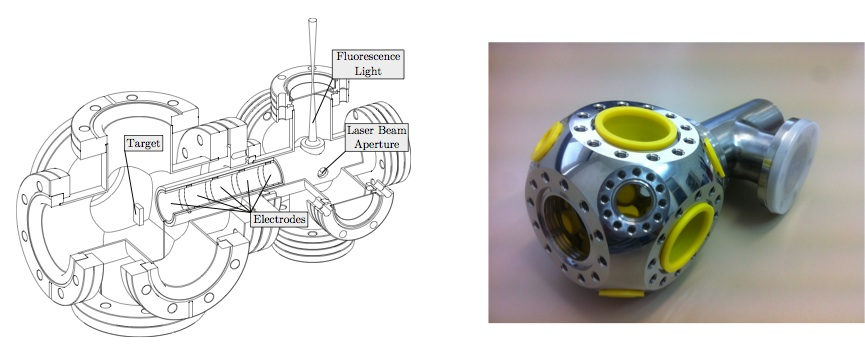
\includegraphics[width=0.99\textwidth]{img/BChamber.jpg}
%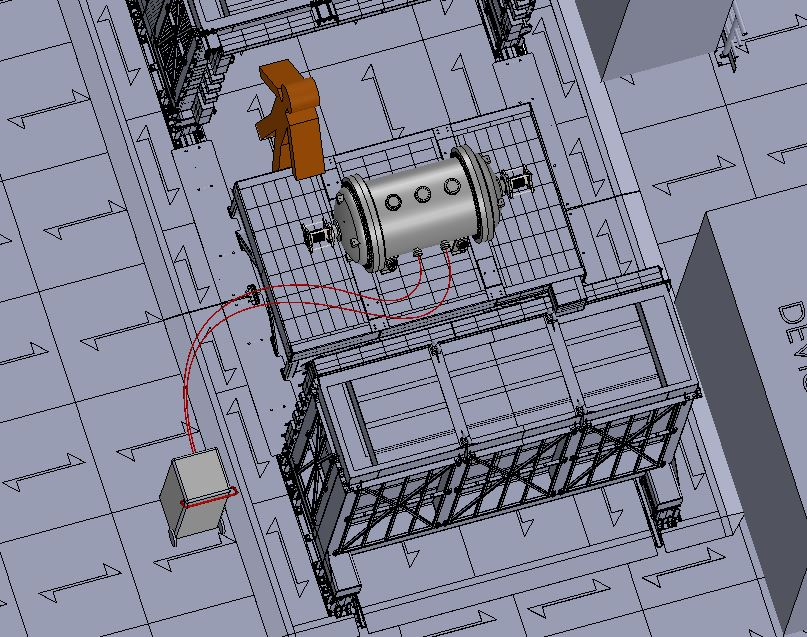
\includegraphics{img/CALIB_LSC_sources.jpg}
\caption{\small Left. A diagram of the chamber for the \BATA\ prove-of-concept experiments: right: the camber, built at IFIC, and ready to be installed at CLPU.}
\label{fig:chamber}
\end{center}
\end{figure}

The \BATA\ subproject will focus in the R\&D program needed to clearly establish the feasibility of tagging (e.g., detecting) the barium (Ba$^{++}$) ion produced in the double beta decay of xenon. Demonstrating that an efficient detection of barium is possible in an \HPXE\ would imply that the NEXT technology could be upgraded to the ton scale while at the same time reducing the background by two or more orders of magnitude, resulting in a virtually background-free experiment with enormous possibilities of hitting a discovery. 

The \BATA\ program involves a set of proof-of-concept experiments. It also proposes the developments of a 4.1 $\mu$m laser, needed for the deshelving of the metastable state. An attractive feature of such laser is its wide range of scientific and technological applications. CLPU is specially well suited to develop the technology.

The different objectives of this subproject are, therefore:

\begin{itemize}
	\item \textbf{Proof of principle experiment with Ba ions generated by means of an electrical discharge.}
In a first round of experiments we will excite resonantly the S$\leftrightarrow$P transition of Ba$^+$ ions generated by an electrical discharge between two barium electrodes and will collect the fluorescence signal of the P$\rightarrow$D transition. Although this generation method is not ideal because several different species different from Ba ions will be generated (e.g., molecules like BaO or clusters), it does not need a major technological development. 

The laser source needed to resonantly excite the $Ba^{+}$ must have a wavelength of 493.5\,nm, not available in commercial lasers. {em The laser source will, therefore be produced at the CLPU}, optimising a tuneable Ti:sapphire laser at 987\,nm to obtain second harmonic generation (SHG) at 493.5\,nm. This setup allows the tuning of the wavelength and control the bandwidth of the laser which is necessary to precisely tune it to the transition frequency (e.g. to correct for pressure broadening and other effects). The IFIC group, on the other hand, has fabricated the test chamber needed for the experiments 
(see Figure \ref{fig:chamber}). 

It is expected that these initial set of experiments will provide valuable information about the population dynamics in Ba$^+$ ions, and the influence of the different homogenous and in-homogenous broadening mechanisms. 
	
	\item \textbf{Proof of principle experiment with Ba ions generated by an ion source.}	
In this objective, in order to get a better approximation of the final conditions of NEXT experiment a source of ions will be designed and constructed at the CLPU. This ion source will be based on selective ionisation and mass spectrometry techniques, and it will allow an efficient selection of the desired target species (e.g, $Ba^{+}$~and $Ba^{++}$). With this setup we will be able to study the recombination process Ba$^{++}\rightarrow$Ba$^{+}$ and decide whether it can be induced by collisions with xenon atoms or requires an additive (see discussion in the objectives of the CALREC subproject). 
	
	\item \textbf{Proof of principle experiment with Ba ions generated by an ion source and with a magneto trap.}	
 In order to better control the experimental conditions, we will repeat the experiment but with the ions now confined in a magnetic trap. This trap will allow us to have an excellent degree of control over the experimental conditions and to approach the conditions that can be expected in the NEXT experiment. For instance we will carry out different measurements comparing the collected fluorescence signal as a function of the pressure of the Ba$^+$ ions and the pressure of the surrounding environment. These measurements are mandatory because the population dynamics is very sensitive to pressure, i.e., to collisions. 
	
	\item \textbf{Proof of principle experiment with an additional laser for deshelving the D state.}
A likely scenario is that the collisional induced decay between the metastable state D and the ground state S is either not effective or too slow for obtaining an appreciable fluorescence signal. In this situation the population is trapped in the metastable state D  and the fluorescence cycle can not be closed. To avoid this difficulty our approach will be to use a second laser to induce a two photon transition (one photon is forbidden by selection rules, between the states D and S, see Fig.\,\ref{fig.BATA}). 

\item \textbf{Development of a state-of-the-art 4.1\,$\mu$m laser}. The laser needed for
deshelving the D state must have a wavelength of around 4.1\,$\mu$m. While small commercial laser system exists in this range, (we will purchase one of them for the experiment described in the previous paragraph), no commercial system will satisfy the conditions of power and stability needed for a real \BATA\ experiment. Furthermore, such a laser, already well in the infrared region, has many potential applications.	

There are only a few laser systems that generate laser emission in the mid-infrared (MIR, from 2 to 10\,$\mu$m). There are lasers that emit in discrete wavelengths as gas lasers ($CO_2$, Xe-HE, He-Ne), chemical lasers (Hidrogen Fluoride, Deuterium Fluoride) and Dye lasers by Raman Shift. All this systems are big and complex, emit in relative low power and are involve the use of dangerous materials (chemicals, flammable gases and/or carcinogenic powders). 

A much more interesting alternative to reach the desired MIR wavelength is the use of an optically pumped solid state laser (OPSSL) system, by means of a specific doping of crystals with metal transition ions. Wavelengths of 2 and 2.9\,$\mu$m are available with $Tm^{3+}$, $Tm^{3+}$-$Ho^{3+}$ and $Er^{3+}$ active ions in crystalline matrices. Recent developments involve doping with $Cr^{2+}$ and $Fe^{2+}$ ions. This should allow to develop a laser system that emits in a broad range: 2.1 to 3\,$\mu$m and 3.7 to 5\,$\mu$m, respectively. Another option is to work with quantum cascade semiconductor systems potentially available from 3.8 to 9.5\,$\mu$m in a discrete range, i. e.  not only continuously. 

To develop a laser system around 4.1\,$\mu$m we need to study and evaluate the best optical parameters of some materials (crystalline matrices or semiconductors) that can be used as active laser materials.  This will allow us to design a laser cavity with the appropriate  optical components and devices (these should work in the MIR region). It will also allow us to maximise the efficiency of the laser system. The cavities are different for systems optically pumped (the case of crystals doped with $Cr^{2+}$ o $Fe^{2+}$) or electrically pumped (as the quantum cascade semiconductors). These cavities can be 2-, 3- or 4- folded mirror configurations depending on the advantages observed during the design using optical and numerical software. The characterisation of the laser emission and other related parameters will allow us  to improve the laser system to use in the NEXT experiment. 

\end{itemize}

%\subsubsection*{\BATA\ subproject: Resources}
%
%For the successful development of this subproject, CLPU will provide the required human and technological resources. CLPU is the centre of reference in Spain regarding laser technology, and takes active part in several international and national projects. The leader of this subproject will be Alicia V. Carpentier who has a well recognised international trajectory in laser-matter interaction. Moreover, {\bf CLPU considers this project of high priority and consequently will offer the collaboration of all the scientific department} consisting of a multidisciplinar team with broad experience in laser technology and development, and laser-matter interaction. 
%
%Furthermore, CLPU will support this project with some of the already operating laser systems in its installation. This is extremely important because such systems usually cost of the order of several hundreds of thousand euros. The human resources needed to operate the laser systems will be provided by CLPU as well. For the construction of the ion source, and taking into consideration the specific requirements of this development, we will apply for an \emph{EXPLORA tecnología} in the 2014 call. 
%
%The budget of this subproject will be dedicated to: a) purchase small equipment for the proof-of-principle experiments; b) purchase a small commercial infrared laser for the initial deshelving experiment; c) develop a state-of-the-art, high power, very stable infrared laser to be used in a large system. It is important to insist that such a laser has many possible applications given the fact that its wavelength is not absorbed by the atmosphere as it lies in what is called the infrared atmospheric window.
%
%
%\subsubsection*{BATA subproject: schedule}
%
%
%

% Los objetivos específicos de cada uno de los subproyectos participantes, enumerándolos brevemente, con claridad, precisión y de manera realista (acorde con la duración prevista del proyecto).
%
% En los subproyectos con dos investigadores principales, deberá indicarse expresamente de qué objetivos específicos se hará responsable cada uno de ellos.
%

\subsection*{\sc Metodología}

%4. El detalle de la metodología propuesta en cada uno de los subproyectos participantes, incluyendo la viabilidad metodológica de las tareas. Si fuera necesario, también se incluirá una evaluación crítica de las posibles dificultades de un objetivo específico y un plan de contingencia para resolverlas.
%

\subsection*{\sc Infraestructuras y equipos}

%5. La descripción de los medios materiales, infraestructuras y equipamientos singulares a disposición de los participantes que permitan abordar la metodología propuesta.
%

\subsection*{\sc Cronograma}

%6. Un cronograma claro y preciso de las fases e hitos previstos en relación con los objetivos planteados en la propuesta en su conjunto.
%

\subsection*{\sc Personal}
%7. Si se solicita ayuda para la contratación de personal, justificación de su necesidad y descripción de las tareas que vaya a desarrollar.

\subsection{\sc IMPACTO ESPERADO DE LOS RESULTADOS/EXPECTED IMPACT}
\subsection{\sc CAPACIDAD FORMATIVA DEL EQUIPO/TRAINING CAPABILITIES OF THE GROUP}
\subsection{\sc IMPLICACIONES ÉTICAS Y/O DE BIOSEGURIDAD/ETHICS AND SAFETY IMPLICATIONS}

\end{document}

%Los resultados de la fase de R\&D de NEXT (financiada por el CONSOLIDER-INGENIO CUP y con importantes contribuciones de los grupos USA) se han traducido en numerosas publicaciones, presentaciones a congresos y charlas invitada (http://next.ific.uv.es/next/talks.html). NEXT ha sido declarado experimento reconocido del CERN y el comité de física nuclear del DOE norteamericano (NSAC) lo cita como uno de los más interesantes del campo (http://science.energy.gov/~/media/np/nsac/pdf/docs/2014/NLDBD_Report_2014_Final.pdf). 
%
%Así, por ejemplo, la vasija a presión ya ha sido construida y los sensores internos (PMTs y SiPMs) ya han sido adquiridos. También han sido adquiridos 100 kilos de gas xenón enriquecido y 100 kilos de gas xenón empobrecido en \XE.
